% Suggested LaTeX style template for Masters project report submitted at the
% Department of Computer Science and Technology
%
% Markus Kuhn, May 2022
% (borrowing elements from an earlier template by Steven Hand)

\documentclass[12pt,a4paper,twoside]{report}
% append option ",openright" after "twoside" if you prefer each chapter
% to start on a recto (odd-numbered) page in a double-sided printout

\usepackage[pdfborder={0 0 0}]{hyperref}  % turns references into hyperlinks
\usepackage[vmargin=20mm,hmargin=25mm]{geometry}  % adjust page margins
\usepackage{graphicx} % allows inclusion of PDF, PNG and JPG images
\usepackage{parskip}  % separate paragraphs with vertical space
                      % instead of indenting their first line
\usepackage{setspace} % for \onehalfspacing
\usepackage{refcount} % for counting pages
\usepackage{upquote}  % for correct quotation marks in verbatim text
\usepackage{float}
\usepackage{wrapfig}


\usepackage[square,numbers]{natbib}
\bibliographystyle{abbrvnat}
\usepackage{url}
\usepackage[colorinlistoftodos]{todonotes}

\newif\ifsubmission % Boolean flag for distinguishing submitted/final version

% Change the following lines to your own project title, name, college, course
\title{Using effect handlers for efficient parallel scheduling}
\author{Bartosz Modelski}
\date{June 2022}
\newcommand{\candidatenumber}{1234N}
\newcommand{\college}{Lucy Cavendish College}
\newcommand{\course}{Master of Philosophy in Advanced Computer Science}

% Select which version this is:
% For the (anonymous) submission (without your name or acknowledgements)
% uncomment the following line (or let the makefile do this for you)
%\submissiontrue
% For the final version (with your name) leave the above commented.

\begin{document}

\begin{sffamily} % use a sans-serif font for the pro-forma cover sheet

\begin{titlepage}
\makeatletter

% University logo with shield hanging in left margin
\hspace*{-14mm}
\includegraphics[width=65mm]{logo-dcst-colour}

\ifsubmission

% submission proforma cover page for blind marking
\begin{Large}
\vspace{20mm}
Research project report title page

\vspace{35mm}
Candidate \candidatenumber

\vspace{42mm}
\textsl{``\@title''}

\end{Large}

\else

% regular cover page
\begin{center}
\Huge
\vspace{\fill}

\@title
\vspace{\fill}

\@author
\vspace{10mm}

\Large
\college
\vspace{\fill}

\@date
\vspace{\fill}

\end{center}

\fi

\vspace{\fill}
\begin{center}
Submitted in partial fulfillment of the requirements for the\\
\course
\end{center}

\makeatother
\end{titlepage}

\newpage

Total page count: \pageref{lastpage}

% calculate number of pages from
% \label{firstcontentpage} to \label{lastcontentpage} inclusive
\makeatletter
\@tempcnta=\getpagerefnumber{lastcontentpage}\relax%
\advance\@tempcnta by -\getpagerefnumber{firstcontentpage}%
\advance\@tempcnta by 1%
\xdef\contentpages{\the\@tempcnta}%
\makeatother

Main chapters (excluding front-matter, references and appendix):
\contentpages~pages
(pp~\pageref{firstcontentpage}--\pageref{lastcontentpage})

Main chapters word count: 467

Methodology used to generate that word count:

[For example:

\begin{quote}
\begin{verbatim}
$ make wordcount
gs -q -dSAFER -sDEVICE=txtwrite -o - \
   -dFirstPage=6 -dLastPage=11 report-submission.pdf | \
egrep '[A-Za-z]{3}' | wc -w
467
\end{verbatim}
\end{quote}

]

\end{sffamily}

\onehalfspacing

\chapter*{Abstract}

Write a summary of the whole thing. Make sure it fits on one page.

\tableofcontents
%\listoffigures
%\listoftables

\chapter{Introduction}

\label{firstcontentpage} % start page count here

\label{section:introduction}
This section introduces and motivates the central problem of this dissertation in \ref{section:thesis}, and provides an overview of the findings in \ref{section:findings}.  

\section{Thesis}
\label{section:thesis}
20 years ago computer processors looked very different than today. The first stock, non-embedded multicore processor has just been released \cite{POWER4Wi47:online} but the customers would have to wait until 2004 to see the first multicore x86 CPU - dual core AMD Opteron \cite{AMDAnnou13:online}. Up to four of them could have been stacked inside HP ProLiant DL585 server. At the time, a revolutionary technology, which allowed continuation of the exponential increase of computational power in chips \cite{mooremulti} in the light of the slowdown of Dennard scaling \cite{Bohr2007}. This technological direction is still relevant today and remains a large driver of performance improvements. Today, a standard dual-socket machine equipped with two stock processors (AMD EPYC 7702 \cite{2ndGenAM1:online}) offers 256 logical cores. In the meantime, the maximum clock speed between these two processors improved by only 20\% (respectively 2.8 GHz and 3.35 GHz for Opteron and Threadripper). Thus, software engineers have strong reasons to try to parallelize workloads. 

Practice shows that parallel programming is far from trivial. Mistakes are common in the daily life of programmers and in research, in algorithms oftentimes claimed to be proven \cite{Norris2013}. This inability to take advantage of parallelism is suggested to have a real impact on the productivity of IT-using sectors of economy \cite{Khan2018}. There is a number of research spaces trying to make parallel programming easier. One particularly important for modern operating systems and runtimes is scheduling. 

A common definition of scheduling explains it in terms of allocating resources to tasks. Justifiably. It captures the essence of the term in a concise and interdisciplinary manner. However, in the context of systems, perhaps, a more illuminating way to think about scheduling is about bridging hardware parallelism and software concurrency. Not long ago, computer could get by with far less advanced schedulers as hardware offered no parallelism. Similarly, workloads used to be less concurrent. With less networking, worse interfaces, fewer programs running on a single computer, more acute cost of context switching, interactivity and fairness were a far smaller concern than they are today. 

This is no longer the case with processors scaling mostly horizontally and evermore complex applications. Thus, this dissertation argues the following thesis. 

\begin{quote}
    Modern hardware is so parallel and workloads are so concurrent, that there is no single, perfect scheduling strategy across a complex application software stack. Therefore, there are significant performance advantages to be gained from customizing and composing schedulers.
\end{quote} 

The first part of the statement is akin to construction of No Free Lunch theorem \cite{Ho2002} for schedulers. While there is a growing body of NFL theorems for optimization problems (e.g. \cite{Wolpert1997}, \cite{Igel2005}), such fundamental results typically formalize knowledge, rather than produce direct guidance for real-world engineering. Therefore, this dissertation aims for a different exposition of the problem, one that analyses practical differences between scheduling policies. It considers widely-used performance metrics and explores the trade-offs between pragmatic scheduling schemes, guided by benchmarks executed on stock hardware. 

The following sections strengthen the thesis from the point of view of hardware parallelism (\ref{section:intr_hardware_par}), software concurrency (\ref{section:intr_software_conc}) and the opportunity presented by OCaml Multicore (\ref{section:intr_ocaml-multicore}).

\subsection{Parallelism}
\label{section:intr_hardware_par}


\begin{figure}
    \centering
    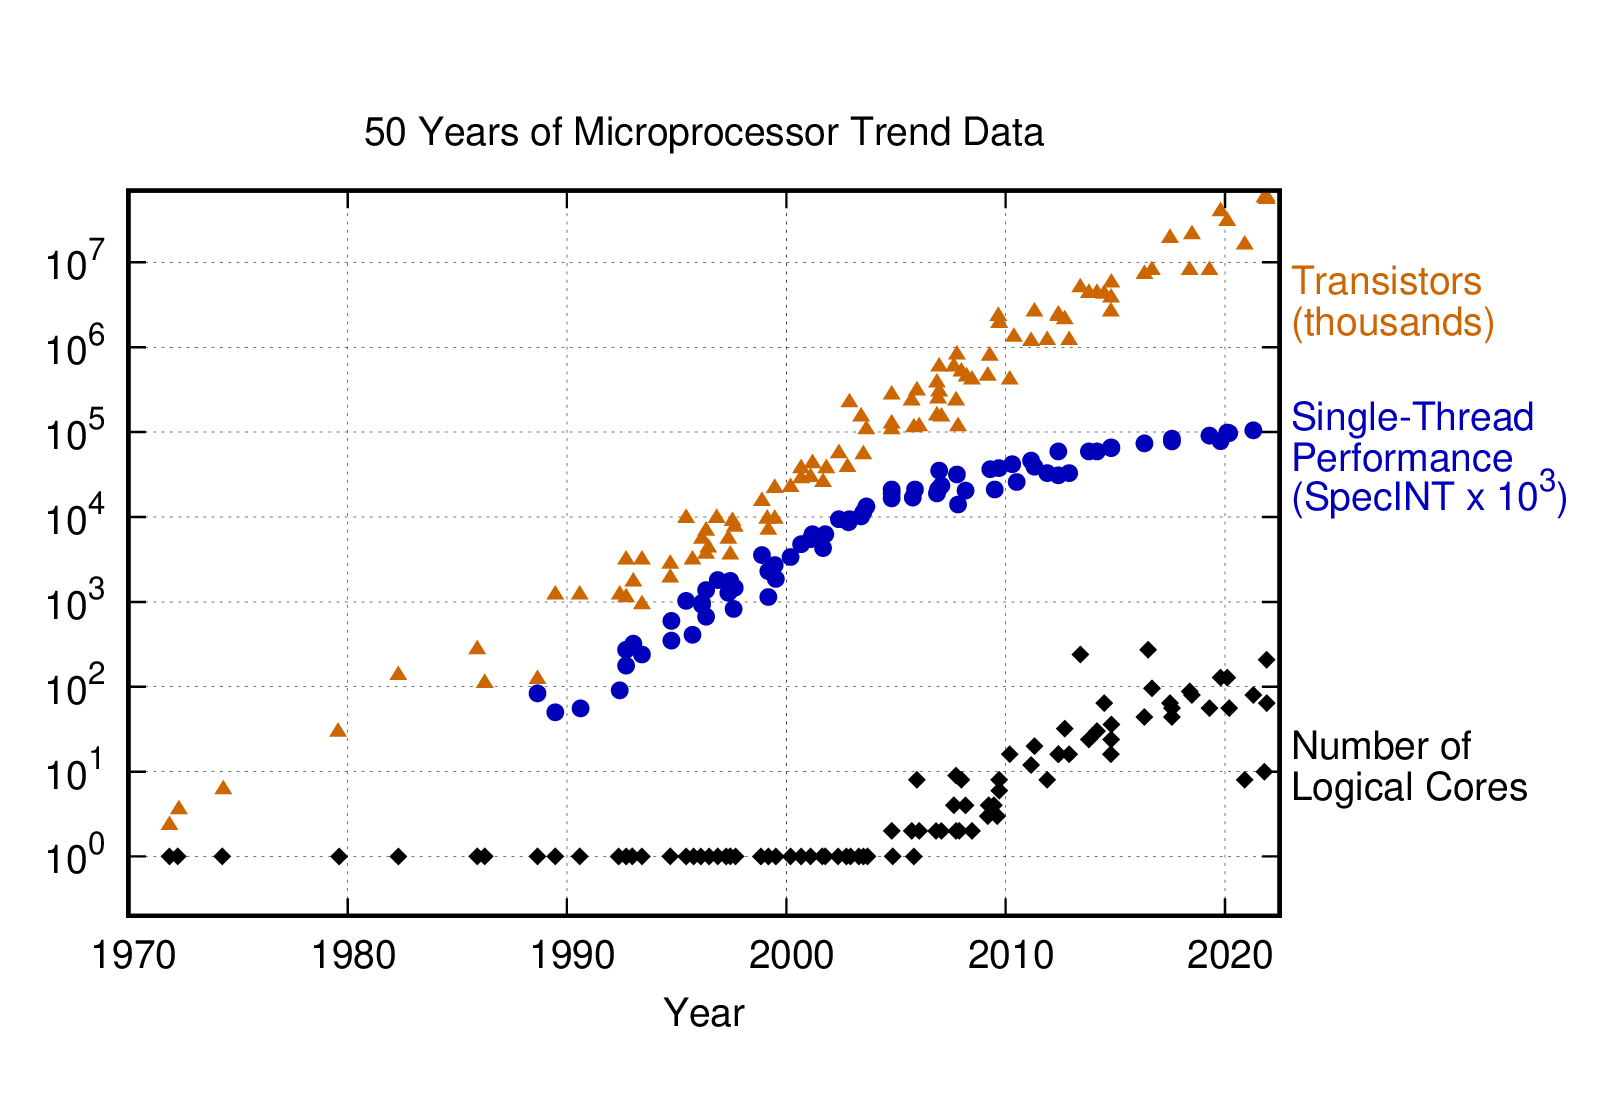
\includegraphics[width=0.85\textwidth]{50-years-processor-trend.png}
    \caption{50 years of evolution of processors. The single-core performance sees diminishing returns but during the last 15 years CPU manufacturers turned to multicore architectures. Figure generated using \cite{karlrupp48:online}.}
   \label{fig:50yrs}
\end{figure}


Moore's law is an observation stating that number of transistors in integrated circuits tends to double every two years \cite{Moore2006}. Around the turn of the millennium, increasing single-core performance at exponential rate was no longer possible due to physical limits. Thus, manufacturers turned to stacking multiple processing units within a single chip \cite{Geer2005}. As shown by figure \ref{fig:50yrs}, the exponential growth of transistors continued, together with exponential increase in cores. While some researches conjecture this trend to slow down \cite{6307773}, \cite{mooremulti}, we still see rapid, if not exponential, growth in this area.

Hence, parallelism is here to stay. Naturally, in contrast with clock frequency increases, schedulers have to be carefully crafted in order to take full advantage of horizontal scaling of the underlying architecture. That's because:
\begin{itemize}
    \item Designs need to evolve as synchronization primitives like locks or atomics do not scale endlessly and e.g. a naive work stealing scheduler may have been good enough on 16-thread Intel Xeon in 2012 but fail to utilize all 128 threads of a contemporary AMD ThreadRipper  \cite{Castello2016}. 
    \item Modern high-core architectures feature non-uniform . Thus, memory latency patterns vary with the topology and scheduling decisions may benefit from taking memory hierarchy into account (e.g. \cite{Drebes2016}, \cite{faverge:inria-00416502}). Moreover, the non-uniformity appears also in consumer products such as Apple M1 or Intel Core i7-1280P. These feature two sets of cores: one optimized for performance and another one for efficiency.
\end{itemize}

\subsection{Concurrency}
\label{section:intr_software_conc}
Workloads become more concurrent and there is a number of reasons behind that. High concurrency is a necessary condition to take advantage of the available parallelism. Compute-heavy application have strong incentives to try to distribute work across multiple cores in the world of stalled single-clock speeds. 

Secondly, the complexity of underlying workload increases as computers become more ubiquitous. There is more useful programs available and the act of composing their executions (to run together) requires concurrency. The programs alone become more complicated. Data-intensive applications \cite{Kleppmann2017-en} require more concurrency as networked portions of the code benefit from scheduling guarantees. 

Finally, concurrency is a convenient tool for expressing certain workloads. Legacy Windows GUI applications are organized around an event loop, which processes inputs from the user. Programmer has to carefully judge the handler logic to never starve the loop and cause the UI to freeze. It turns out very difficult in practise; a typically small IO may be pointed at a network location and take orders of magnitude longer. A simple compute might stall for far longer on an overloaded system. A modern Go application can simply spawn a new goroutine for every handler and rest assured that runtime prevents starvation of the event loop.  

\section{Tools}
This sections describes the system and programming environment used to verify the thesis. 

\subsection{System}
The report aims to investigate runtime scheduling space on a modern, high-core machine. Used system features two AMD EPYC 7702 processors, which gives a total of 128 physical cores and 256 threads. It runs Ubuntu 22.04. For more details, see \ref{section:methods_system}. 

\subsection{OCaml Multicore}

\textbf{Scheduler as a library, scheduler composable}
\label{section:intr_ocaml-multicore}

OCaml is a unique functional programming language, which aims to deliver performance and safety. It found many research and industrial users despite a significant shortcoming for a performance-oriented language - lack of support for multithreading. This confined real-world applications to monadic concurrency libraries such as Async and Lwt, which are troublesome to use: 
\begin{itemize}
    \item \textbf{No runtime support.} Lack of runtime support hurts the development in a number of ways, e.g.: there is no way to efficiently switch between tasks, tracing becomes harder as there is no real notion of separate threads and stacks. 
    \item \textbf{Blocking.} Combine single-core with lack of preemption and any single CPU-intensive or blocking call is prone to cause chaos by starving other threads: cause network timeouts, delay timers, etc. On the surface, there is no qualitative difference with multicore as any \textit{n} non-preemptive threads can by blocked by \textit{n} misbehaving task. But in practise multicore is far safer. Firstly, developer may isolate low-latency tasks on a different pool, allowing for more relaxed programming elsewhere. Secondly, a multicore runtime may feature a guardian thread, which spawns new OS threads whenever needed \cite{golang}.
\end{itemize}

Nonetheless, after years-long effort, multicore support has been recently merged into the main tree. Thus it is a favourable time to take a closer look at lightweight threads schedulers. Significant changes to existing schedulers are notoriously slow and troublesome, as even subtle differences to scheduling policy may expose bugs in existing programs. During my industrial experience, the only way to deal with such a change was having developers manually verify the code and re-do the testing. Incidentally, both methods are known to be bad at finding bugs in multiprocessing. This research project, however, is likely to contribute to the actual design and implementation of OCaml scheduler. 

Finally, Multicore OCaml is a particularly interesting object of study as it includes a number of novel solutions. Common programming languages either include threading support, which is tightly coupled with the language itself, or offer no support and, thus, library-schedulers cannot offer much beyond simply running scheduled functions in some order. OCaml, on the other hand, features fibers and effects. Together, they allow writing a direct style, stack-switching scheduler as a library. Further, OCaml allows composing schedulers. A much-needed mechanism for executing diverse workloads with portions having different optimization criteria \cite{Tennenhouse89layeredmultiplexing}.


\section{Findings}
\label{section:findings}

\todo{fill in}

\chapter{Background}


This section begins by describing the general problem of scheduling, key concepts and two modern real-world runtime schedulers (\ref{section:background_schedulers}). Afterwards, it describes the tools of choice: important properties of OCaml programming environment (\ref{section:background_ocaml}) and details of fine-grained multicore programming (\ref{section:background_multiprocessing}).

\section{Scheduling}
\label{section:background_schedulers}

Scheduling attempts to assign resources to tasks in a way that optimizes some metrics \cite{Pinedo2012}. The problem itself is not limited to computer science and arises in a number of areas, e.g. organization management. In the case of computer science, it stems from a very fundamental need to compose executions of multiple programs. However, supporting such a model of execution is not trivial. Instructions of multiple programs are inherently impractical to compose, since they all write and read the same registers. In effect, composition is achieved by interleaving executions of multiple programs, and a special mechanism to hide existence of these pauses by saving and restoring state. This leaves us with a clear-cut scheduling problem as there is a need for a holistic decision-making process to determine, which program runs when and for how long. This decision-making perspective is illustrated by figure \ref{fig:sched-graph} and such a model of the problem will be helpful to keep in mind throughout the rest of the report. 


\begin{figure}
     \centering
     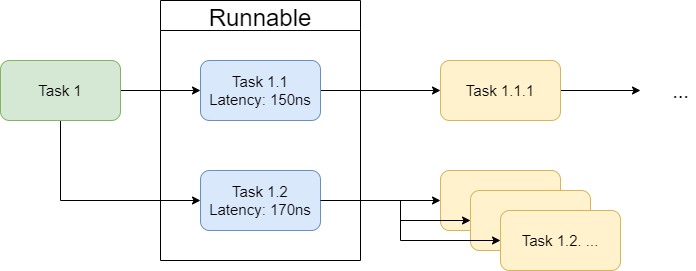
\includegraphics[width=0.85\textwidth]{scheduler_graph.png}
     \caption{A simplified graph of fine-grained tasks, which scheduler attempts to traverse in order to terminate. Green box represents executed task, blue boxes are currently enqueued tasks. The orange boxes are tasks that are going to be scheduled once their parent execute. They are not visible to the scheduler at the moment. This graph shows how little is actually known about the tasks, and scheduler-traps in the shape of infinite-depth subgraphs, which are prone to cause starvation.}
    \label{fig:sched-graph}
\end{figure}


\subsection{System Threads}
\label{section:system-threads}
System threads are a fundamental OS feature, which allows to detach the number of synchronous executions from the number of processing units. All kinds of program grew to rely on this abstraction heavily. For example, Google Chrome spawns a single process per tab \cite{Howwebbr64:online}, and depending on the logic, each such process spawns additional threads. This aggressive acquisition of resources leads to smooth operation of the web browser but puts significant pressure on the operating system, which has to ensure that in the sea of threads everything gets a fair share of the CPU time and their individual objectives are achieved, e.g. a heavy web browser and light but latency-sensitive audio driver.



\subsection{Lightweight Threads}
\label{section:lightweight-threads}
System threading provides the fundamental mechanisms to execute concurrent workloads across parallel hardware. But programmers need to be wary of designed computations as the cost of interacting with kernel is non-trivial. It may vary from mode switching to full syscall overhead. System call logic requires a number of things to happen (e.g. context switch, capability check, audit), which thwart the cost of a small task. Thus, the performance of highly concurrent workloads suffers significantly.

This is inconvenient for the developers. Spawning little concurrent tasks is the natural way to express many common server-side workloads, e.g. processing HTTP requests. Therefore, language designers started to construct lightweight threads, what stands for threading implemented entirely in the user space. They aim to be very cheap to use and they do deliver on that promise. Context switch in Go requires saving and restoring just 3 registers \cite{gorout_vs_os_thread}. In OCaml only 2 \cite{Sivaramakrishnan2021}. Conversely, a system scheduler needs to save and restore \textit{all} registers, and perform mode switching \cite{gorout_vs_os_thread}. Therefore, lightweight threads are naturally better suited to support fine-grained concurrency. The next section touches on a disadvantage of not having access to privileged mode \ref{section:preemption}. 

\subsection{Preemption}
\label{section:preemption}

Preemption is the ability to suspend other tasks without any cooperation on their side. It is a cornerstone of modern OS-level scheduling, in which each program is assigned its quantum of CPU time. Once the quantum is used up, scheduler forcibly ensures other programs get to run. Preemption is a necessary condition to keep the system stable in the world with imperfect and malicious programs. In practise, preemption has more profound consequences. Individual programs no longer have to worry about their composition with others. They may cooperate but ultimately, all decision-making is done by the privileged scheduler, which is able to make more holistic decisions. 

Nevertheless, true preemption is not possible as a pure software solution. Operating systems rely on the hardware support for privileged mode and interrupts. After all, if preemption was not restricted, a single erroneous or malicious application could completely destabilize whole system. Alternatively, running runtime of business logic within the kernel is not acceptable as such application threatens entire infrastructure if compromised. This makes true preemption inaccessible to lightweight threads for security reasons. Moreover, even if there was a safe mechanism to allow true preemption without elevating preemptor into privileged mode, such mechanism might defeat its purpose. Lightweight threads aim to be very cheap and that conflicts with using full OS-level context-switching mechanisms.

Different programming languages and libraries deal differently with this limitation. Particular approaches are discussed in further sections (\ref{section:rel-work-go}, \ref{section:rel-work-rust}).

\subsection{Work stealing}
\label{section:background-work-stealing}
Work-stealing is an extremely widespread concept applicable to all kinds of multicore scheduling. It has been introduced at least 40 years ago \cite{Blumofe1999} and remains used in some of the most cutting edge schedulers, e.g. Completely Fair Scheduler (the default scheduler in Linux) \cite{linux_cfs}, Cilk \cite{Blumofe1995}, Go \cite{golang}.

Work-stealing splits the global work queue (in the FIFO case) into a number of local, per-CPU runqueues. Each processor strongly prioritizes its own runqueue; namely, it will enqueue and dequeue elements from its own structure as long as it is possible. This alone is similar to a number of unrelated processors, actual distribution of work happens when the impossibility criterion is met. If enqueue is impossible (due to lack of space), owner can either resize the runqueue or transfer some of the work into a global overflow queue. If dequeue is impossible (due to lack of items), processor chooses a different processor at random and steals work from the victim, thus balancing the load. There is a number of benefits flowing from such organization. \begin{itemize}
    \item \textbf{Less synchronization and faster hot path}. Since local runqueues are single-producer, the enqueue operation needs little synchronization. Likewise, local dequeue operation only need to synchronize with stealers making it fast as well. 
    \item \textbf{Low contention}. Whenever load on the system is high, processors converge to using their own queues, thus eliminating any need to compete with others for work.
    \item \textbf{Locality}. Children tasks are likely to execute on the same processor as their parents, what maximizes the locality and improves overall performance.
\end{itemize}

\label{paragraph:deque}
Chase-Lev deque (double-ended queue) \cite{Chase2005} is one of the notable, classic work stealing implementations. Its design is similar to the example describe above but while steal remains FIFO, local insertions and removal follow LIFO order. It aimed to minimize required synchronisation, since local thread operates at one end of the structure and steal at the other but also, although not recognized by the authors, it improves locality of the workload \ref{section:approaches}. 

\section{Multiprocessing}
\label{section:background_multiprocessing}

Multiprocessing is a crucial technique to take advantage of the modern processors. There is a number of multicore programming paradigms, each providing different trade-off between safety and performance. While it is rarely the case in software engineering practise, schedulers are critical enough to fully prioritise the latter criterion, and choose lock-free programming. 

This section introduces key multiprocessing concepts with a focus on the lock-free perspective. 

\subsection{Amdahl's law}
As already discussed, taking advantage of parallel hardware requires extra engineering effort. The actual amount of effort varies wildly between tasks. In some cases parallelization is trivial and almost boils down to using relevant threading API, e.g. computation of five independent hashes. In fact, system might automatically parallelize a computation specified by \textit{List.map} \cite{OCamllib90:online}. 

However, on the other hand of the spectrum lie programs, for which parallelization yields marginal or no benefits. It is enough to slightly tweak the previous example to show that. Assume computation of a chain of 5 hashes, wherein each hash depends on the output of the previous one. In such a case, the hashes themselves need to happen in a sequential manner. There might still be opportunity for parallelization but it depends strictly on implementation of the hash operation. Moreover, even if hash operation is very parallelizable, the synchronisation will need to happen before and after every hash operation in the chain (10x), rather than just at the beginning and end of the workload. 


The speedup coming from parallelization is described by Amdahl's law \cite{art_of_mult}.

\begin{center}
$Speedup = \frac{1}{1 - p + \frac{p}{n}}$
\end{center} 

Where \textit{n} is the number of processors and \textit{p} portion of the program that is parallelizable. The law puts a strict bound on the gains coming from using multiple processors and hints why adding more cores yields diminishing returns, as observed in the latter sections. Namely, doubling the number of processing units halves the time spent in parallelizable portion of the workload. Thus, gains on parallelizable portion rapidly become smaller than any non-trivial sequential part of the program. 

\subsection{Lock-free algorithms}
Lock-freedom characterizes algorithms, which guarantee that at least one of many threads is going to terminate in a finite number of steps \cite{art_of_mult}. This is not the case with locks; if thread holding a lock is not scheduled then no one is allowed to make progress. Lock-free algorithms are built with the same low-level primitives, that are used to build high-level blocking synchronization, but here they are applied to the problem at hand. Thus, absence of explicit lock objects does not guarantee lock-freedom, as in theory, blocking behavior can be reimplemented from scratch. 

The main advantage of using lower-level primitives, atomic operations, comes in the form of better control over synchronisation, which may translate into better performance. Naturally, performance improvement is not guaranteed; contentious lock-free algorithm may scale much worse than an alternative implementation based on high-quality locking. 

\subsection{Atomic operations}
Atomic operations are hardware-supported instructions, which guarantee synchronized, indivisible execution. They are mostly non-blocking and tend to operate on at most one processor word. Actual usage and implementations vary between architectures but languages typically provide a unified interface. So is the case with OCaml. This project relies primarily on two atomic operations:
\begin{itemize}
    \item \textbf{Compare and swap}. CAS takes 3 arguments, one variable (memory address and two values: old, new. If the variable equals the old value, then it gets updated to the new value in one step. Success or failure are reported to the caller.  
    \item \textbf{Fetch and add}. FAD takes two arguments, one variable (memory address) and an integer value. The integer is added to the variable and prior value is reported. FAD always succeeds.  
\end{itemize}

Both operations have similar latency when applied to the same use case \cite{fad-cas-speed}. CAS has the benefit of being much more general but at the cost of potentially having to retry. It is worth pointing out, that these operations essentially push the burden of synchronisation to the microarchitectural level but it remains non-trivial. Atomic operations may still take one or two orders of magnitude more cycles than their non-atomic counterparts and most common instructions. 

Implementations of atomic operations may allow or forbid certain kinds of memory reordering \cite{memoryor11:online}. OCaml atomics only come with sequential consistency, which is the strongest restriction. Sequential consistency forbids any reordering across an atomic operation. Therefore, memory order relaxations are not further considered in this report.

\subsection{Linearizability}
\label{section:linearizability}
Linearizability is a property of execution trace, which states that all actions can be recomposed into a correct, sequential history. It is crucial whenever operations execute in parallel, be it in a distributed system or on architectural level. High level concurrency primitives such as locks help to achieve this property trivially; if relevant state is protected by a single lock then any functions linearize since they are forced into sequential order by the very lock. However, such coarse-grained primitives may leave performance on the table. 

When performance is the priority, a common approach is to try to distribute the state to allow many agents to act in parallel. Here, linearizability is easy to involuntarily give up, and becomes a critical property to watch. For example, design of a queue does not generally prohibit enqueuer and dequeuer to operate from operating independently on different ends. Such behavior can be achieved using atomic operations to modify \textit{head} and \textit{tail} indicies, what effectively doubles the throughput offered by lock. However, suddenly a simple size function \textit{tail - head} may produce gibberish output as it no longer linearizes. Independent reads of \textit{head} and \textit{tail} can observe respective values from two different states and compute a particular \textit{tail - head} value without the queue ever being that size.


\subsection{DSCheck}
\label{section:background_dscheck}
Writing concurrent programs is an error-prone process. This is true for all kinds of applications but in particular if they use the lowest level sychronisation primitives, atomic operations. Humans are not good at the kind of precise reasoning required to deal with super-exponentially increasing number of interleavings as more functionalities are added and state becomes more fragmented. Generally, there is no solution to this difficulty. Commonly, academics attempt to write formal proofs for the code, which is also a non-trivial process and have been found to let errors through (e.g. \cite{Norris2013} disproved \cite{correct_and_efficiect_deque}). 

CDSChecker \cite{Norris2013} is a novel approach to verification of lock-free algorithms. It lets the user automatically validate all possible interleavings of a lock-free algorithm, which is extremely helpful in overall validation of the code and tracking down rare race conditions (e.g. occuring a few times in a million executions of tight loop designed to expose such race \cite{litmus}). Moreover, CDSChecker does not require building any model of the code, which could be incorrect, but uses the core implementation of algorithm with shadowed atomics library. 

Core lock-free data structures of this dissertation have been validated using CDSChecker's adaptation to OCaml - DSCheck \cite{sadiqjds97:online}. 

\chapter{Related work}

Scheduling is omnipresent in computer science. It may happen at multiple levels simultaneously: data-center orchestration \cite{NomadbyH95:online}, OS-level threading (\S\ref{section:system-threads}) and runtime threads (\S\ref{section:lightweight-threads}). The field is very rich in literature and applications. Therefore, instead of summarising all the related work (which would be beyond the scope of this report), this section takes a close look at the design of two modern runtime schedulers. Project work and design decisions tie back to this review. 

The first analyzed runtime is part of the Go programming language (\S\ref{section:rel-work-go}). The excellent support for concurrency is one of its main features. Just like OCaml, it is a high-level language with features like garbage collection. However, OCaml also strives strongly to maintain high-performance, does not feature preemption or a built-in runtime scheduling. Therefore, the second reviewed scheduler is Tokio (\S\ref{section:rel-work-rust}), which is a Rust library. It covers all of the mentioned discrepancies.

Finally, OCaml's unique features for supporting concurrency and parallelism are discussed. 

\section{Go}
\label{section:rel-work-go}
Go is an imperative programming language, which aims to be the language for building distributed systems. The first sketches of Go were created by senior Google engineer, heavily drawing on company's extensive experience with building complex backend applications. Go features a deeply integrated support for lightweight threads, called goroutines, whose design was central to the language since its very beginning.

Go standard library adds a significant amount of machinery on top of the POSIX thread interface. Goroutine is quite flexible in that it can be a short-lived task or a long-running process, since the compiler automatically inserts statements returning control to the scheduler in strategic places, like function entry or loops. In contrast with typical OS threads, Go works hard to let developer schedule new routines as freely as possible, allowing hundreds of thousands of them to be executed concurrently thanks to e.g. marginal memory footprint - 2KiB per routine at initialization, while OS threads costs 1MiB (although the memory is virtual). 

On the surface, Go features a classic work stealing scheduler with local queues and steal-half operation to distribute work. There are, however, significant differences. Goroutines are scheduled on a \textit{processor} rather than worker (OS thread). This decoupling improves remarkably over a naive architecture with runqueue per OS thread. Firstly, task may not be able to make progress if in a system call or a synchronization primitive. In such a case worker constitutes the minimal state that \textit{processor} has to park if blocked and unpark if runnable. Secondly, attaching runqueue to a processor maintains the local invariant (even though runqueue changes hands) and keeps the overall number of queues much lower. Thanks to this rotation there is no tasks lingering in inactive runqueues and necessitating more stealing. On the other hand, if worker runs out of work and decides to steal there is less fragmentation and lower chance of selecting other empty queues. Finally, with such a design autoscalability emerges very naturally as it boils down to minimizing the number of runnable workers within available resources. Runqueues have constant size of 256 items and any extra items are pushed into a global locked queue \cite{goprocgo7:online}. 


\section{Tokio (Rust)}
\label{section:rel-work-rust}
Rust is another modern imperative programming language. It encompasses a much different philosophy than Go. Historically, performance and safety were a trade-off. For example, memory management was either manual (error-prone, zero-overhead) or handed to the garbage collector (safe, non-trivial overheads). Rust strives to achieve both: safety and performance on par with C++. It applies a number of novel ideas, e.g. ownership system, but they typically come in the form of zero-cost abstractions or static analyzers as adding runtime overheads would quickly make the goal of matching C++ performance unattainable. 

Therefore, threading in Rust's standard library largely maps to OS threads and leaves building out more advanced management to the user. One particularly successful attempt is Tokio \cite{TokioAna8:online}. An external library, which provides multithreaded runtime and an asynchronous version of standard library.

Just like Go runtime, Tokio also relies on work stealing to share work. However, it does not abstract out OS threads and relies on a much simpler scheme with a single worker per OS thread and number of OS threads corresponding to number of processing units. As the total number of threads is limited and external library cannot do preemption, such a scheme is prone to liveness issues. Thus, Tokio provides a special spawn\_blocking call to spawn new OS threads on demand for blocking or CPU-intensive computations. Tokio also features a global overflow queue if there is no space in the local runqueue. Notably, Tokio relies on a CDSChecker-inspired lock-free validation as well - Loom \cite{tokiorsl53:online}.

\section{OCaml}
\label{section:background_ocaml}

As touched on in \ref{section:intr_ocaml-multicore}, OCaml introduces a new flavor of multiprocessing. It brings a number of benefits, but the most important one from the point of view of this dissertation is decoupling of scheduling and runtime \cite{stephen_effective_nodate}. In simple words, a developer of an external OCaml library now has the ability to write a powerful, built-in-like runtime scheduler without requiring any changes from the standard library, the runtime system or OCaml compiler. The rest of this section describes mechanisms enabling this decoupling and other notable features of Multicore OCaml.

\subsection{Threading}
\label{section:fibers}
Starting with version 5.0, OCaml will offer access to OS threading through the domain interface. System threads are heavy due to high memory footprint, the overhead of systemcalls and context-switching. Domains are similar, in that a single domain consist of an OS thread and additional OCaml structures such as local minor heap \cite{Sivaramakrishnan2020}. Generally, domains offer course-grained parallelism and they are optimized for the number of domains to not exceed number of processing units \cite{Concurre37:online}.

To use system threads efficiently, we also need concurrency. Historically, OCaml did not provide any explicit support for writing concurrent programs. Thus, developers using Lwt/Async were forced to divide programs into small functions, which are then scheduled dynamically and executed on the same stack. 

Multicore OCaml features fibers - light, heap-allocated, resizable stacks. They are non-preemptible. Number of concurrent fibers is limited by memory and may exceed number of logical cores by orders of magnitude without any issues. Furthemore, context-switching between fibers is extremely cheap. It requires saving stack and exception pointers of the fiber and loading ones of the target frame \cite{Sivaramakrishnan2021}. Therefore, they are a perfect foundation for efficient, fine-grained concurrency. 

\subsection{Effects}
\label{section:effects}
Effects represent a novel way of modelling not just concurrency but all kinds of computational effects. The concept is a product of research on theory of computation \cite{Pretnar2015} and, even though the formal underpinnings are far beyond the scope of this report, it is introduced the easiest by analogy. 

An imperative programmer may consider it a generalisation of exceptions \cite{Brachthuser2020}. Using exception language, effects allow throwing an exception (performing effect), processing it, and optionally returning to the location of throwing (continuation) to resume execution. For a functional programmer, effects provide similar capabilities to monad transformers but in direct-style, without imposing monadic form on \cite{Sivaramakrishnan2021}. This is especially important for concurrency, as with Async and Lwt real-world applications end up having almost all code written in the monadic form to prevent liveness issues. 

In the case of threading, effects provide a composable mean of stopping and resuming execution. Once effects handlers are set up higher up the stack, any function may perform a yield effect, which immediately returns the control back to the handler. Up until now, the logic is implementable with exceptions. However, the handler also receives a \textit{delimited continuation}, which resumes execution of the yielding function. In the case of a scheduler, handler may put received continuation into a queue, take the oldest element and resume it instead. This logic is implemented efficiently using fibers described in the previous section (\ref{section:fibers}). Whenever effects handler is set up, it instantiates a new fiber for contained logic. If said logic performs an effect, said fiber is unchained from the top of the stack and a new one is created to execute the handler. Naturally, this harmony is by design, and fibers and effects have been strongly optimized to support high-performance concurrency. 

\label{paragraph:ocaml_preemption}
In the current shape, effects do not mix with preemption. True preemption is limited to OS-level scheduling. There is no way around this restriction as true preemption requires special privileges and it is not acceptable for ordinary applications to have them due to security concerns. In the case of Go \ref{section:rel-work-go}, runtime simulates preemption by having compiler automatically insert optional yields into strategic places (checkpoints) in the code. Similar solution does not really fit OCaml out of the box because it would pollute entire program with Yield effect, what defeats the purpose of effects system. In Go, such logic is hidden within the runtime and compiler. In the case of OCaml, suddenly pure or even no-op functions would emit effects. 

\subsection{Garbage collection}
\label{section:gc}
OCaml features a new garbage collector created with multicore in mind \cite{Sivaramakrishnan2020}. It has two generations: local minor heaps and a shared global major heap. Both minor and major heap collections require stop-the-world pause. The minor collection is fully parallel \cite{Sivaramakrishnan2020}.

\subsection{Domainslib}

OCaml ecosystem already has a scheduler endorsed by the core developers \cite{ocamlmul59:online} - Domainslib. However, multicore OCaml has not been widely adopted yet and thus, Domainslib is not as mature as in the case of other ecosystems. The design of Domainslib closely follows classic deque (\S\ref{paragraph:deque}). Therefore, Domainslib is not dissected as one of the state of the art schedulers but its performance is compared against this project in (\S\ref{section:result_with_domainslib}).

\chapter{Design}
This chapter describes the design space of a scheduler. First, \S\ref{section:objectives} states the desirable properties and metrics to evaluate scheduling policies. Afterwards, major approaches are described and other design choices are discussed in the remainder. 

\section{Objectives}
\label{section:objectives}
During the early days of computing, throughput of a system was significantly more important than the interactivity. After all, user interface could be as minimal as punch cards for input and a printer for output. Properties like latency or fairness were in the hands of human operator. Over time, however, computers became ubiquitous and networked. People and businesses started to depend on automatic processes terminating timely and reliably. In fact, major software companies such as Amazon, Google have measured the direct impact of latency on their revenue \cite{Kleppmann2017-en}.

Therefore, in line with the literature (e.g. \cite{8057206}, \cite{latthrough}, \cite{Sun2021}), a scheduler should aim to achieve high throughput and some desired latency characteristics. Typically low tail latency.
\begin{itemize}
    \item \textbf{Throughput}. A scalar value of tasks (or some other unit of work) processed over a time unit.
    \item \textbf{Latency}. The distribution of processing time of tasks over some workload. Naturally, while queueing theory deals with entire distribution, in software engineering practice it is more common to select one or multiple percentiles as the key metrics. For example Amazon chose to optimize 99.9th percentile of latency and deemed higher ones not cost-effective \cite{Kleppmann2017-en}. But a test-suite of a distributed system may consider both 99.9th percentile and median to have a better picture of the system, while a low-latency market maker may focus primarily on top 20\% since those are the orders that win the race with their competitors - for everything slower the actual size of the delay is not important. 
\end{itemize}

Preemptive schedulers may also explicitely prioritize fairness. Naively, the lower latency the more fair scheduling, however, this does not hold if jobs have different sizes. For example, a scheduler may prefer to starve a rare long-running job rather than keep thousands of small tasks waiting, since the latter is going to have a higher impact on mean or (sufficiently small) nth percentile latencies. However, as OCaml does not feature any preemption mechanisms (\S\ref{paragraph:ocaml_preemption}) and the CPU time is effectively specified by the developer, the schedulers developed in this project treat all tasks as drawn from the same distribution. As discussed further in (\S\ref{section:design-staged}), staged architecture does allow developer to more explicitely choose between fairness, latency and throughput. 


\section{Benchmarks}
This section describes the three main benchmarks used to evaluate different scheduler designs on realistic workloads with respect to described objectives (\S\ref{section:objectives}). Each benchmark aims to simulate the true characteristics of the core of each workload (e.g. branching factors, dependencies between tasks, memory patterns) but at the same time aggressively mock all dependencies such as networking and other IO. This significantly reduces noise in the benchmarks and improves replicability. 

\subsection{Packet processing}
\label{section:background_packet-processing}
TCP is a backbone of the internet as we know it. It is used by countless applications, from the world wide web to low-latency trading infrastructure. Thus, the algorithms for processing TCP packets became very sophisticated. At any step they tend to only parse the parts of the packet that are necessary to proceed. Such lazy behavior is critical for performance and security.

Therefore, the first benchmark imitates a TCP server, e.g. webserver. Firstly, it accepts a packet and spawns a lightweight thread for its processing, which in turn scans for newlines. The first necessary step in order to do more selective and possibly parallel parsing afterwards. 

\subsection{Audio mixer}
\label{section:bench-audio-mixer}
Telecommunication is a relatively low latency endeavour. Research in human-computer interaction generally recommends keeping latency of (any) response below 100ms for it to feel instantaneous (\cite{Miller1968}, \cite{Amin2013}). Beyond that, users begin to notice the delay and the experience deteriorates. \cite{voip-latency} focuses on mouth-to-ear latency in softphones (software phones) and classifies everything below 150ms as excellent, 150ms-300ms good and over 300ms as poor. 

While 150ms round-trip time may seem like an undemanding deadline for a modern server but there is a lot that can go wrong (and goes frequently, as we have experienced during the pandemic). 
\begin{itemize}
    \item \textbf{Network latency}. In practise vast majority of the RTT budget is consumed by the transport. Packet may have to cross multiple carrier networks or simply a large geographical distance. In practise, the less latency is imposed by the server the better average user experience. 
    \item \textbf{Throughput}. Typical VoIP call-leg sends 20ms frames, each containing a few hundred bytes of audio. In my professional experience, a typical FreeSWITCH \cite{Maruzzelli2017-ou} installation was expected to handle up to 1000 concurrent calls without quality loss. 1000 concurrent calls with 2 legs each and bidirectional media means processing 100k packets a second. Each with a real deadline much smaller than the mentioned 150ms. 
    \item \textbf{Audio complexity}. Moreover, standard VoIP signalling protocol SIP allows every participant of a conference to negotiate different codecs. Thus, the server has to decompress all incoming audio, mix it together, compress, and only then send out. In the case of mentioned FreeSWITCH, each call-leg has a separate thread for IO and codecs, and another one per conference to mix audio. That results in audio being passed around and buffered a lot, potentially causing contention.   
\end{itemize}

Thus, the second benchmark imitates a VoIP server with a number of conferences and participants, and FreeSWITCH-like \cite{Maruzzelli2017-ou} audio-processing, audio-mixing threads. This benchmark aims to simulate an enterprise application with extremely complex scheduling patterns and a perhaps not perfectly optimized code, where individual threads frequently need to yield to wait for others.

\subsection{Binomial option pricing}
\label{section:bench-option-pricing}
The last benchmark delves into the world of finance. The livelihood of trading shops depends on their ability to accurately and timely price instruments. 

\todo{finish me}

Moreover, binomial option pricing requires an interesting dynamic processing computation. It builds a lattice of possible future prices and walks it backwards to propagate expected options payoff taking interest rates into account. The computation is non-trivial to effectively parallelize. 

\section{Ordering}
\label{section:approaches}
This section describes the core ordering problem in scheduling.

\subsection{FIFO and LIFO}
\label{section:ordering}
First in, first out (FIFO, also FCFS) regime assumes running tasks in the order of arrival. Effectively, that corresponds to traversing the graph in figure \ref{fig:sched-graph} in a breadth-first manner. FIFO is commonly used in the real-world schedulers. As evidenced during writing of this report, it is extremely robust. The mechanism of always taking the oldest element naturally acts against high latencies and starvation. The latter, arguably, being one of the most undesirable failure modes in a scheduler. Thus, user can use a FIFO scheduler fairly freely and expect no adverse effects beyond a potential performance penalty. Moreover, additional features tend to be easier to implement (e.g. \S\ref{section:yield}) as this kind of traversal remains robust even with minor reorderings caused by stealing, overflow structures, incautious workloads, etc.

Last in, first out (LIFO) order takes the opposite approach and always attempts to schedule the most recently added task. It results in a depth-first search traversal of the DAG, which hints at its potential for starvation if at least one of the scheduled workloads consist of an infinite graph. The main advantage, however, lies in LIFO scheduling respecting the principle of locality. Tasks tend to be related to each other and by running the most recently scheduled task, the scheduler maximizes the chance that required data is still in cache. Since memory is hierarchical, the benefits should be noticeable for a number of tasks executed in order and for a wide range of memory requirements. 

These two fundamental strategies highlight the common trade-off between throughput and latency in scheduling (\S\ref{section:objectives}), which stems directly from policy on the lowest level: prioritising either oldest task (for latency) or newest (for locality). 


\subsubsection{Fairness revisited}
\label{section:fairness-revisited}

\begin{figure}
    \centering
    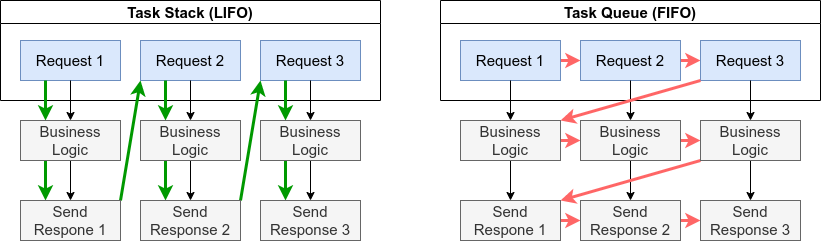
\includegraphics[width=1\textwidth]{FIFOLIFO.png}
    \caption{The figure shows two ways to traverse tasks graph. Boxes with blue shade represent task physically present in run queue, run stack. The grey boxes constitute tasks that are going to be spawned by their respective parents. To simplify, assume that every task is drawn from the same distribution. In such a case, requests processed using FIFO order terminate at timestamps 7, 8, 9, while using LIFO at 3, 6, 9. Thus, even though FIFO optimizes per-task latency, the latency of actual requests favors LIFO.}
   \label{fig:fifo-lifo-latency}
\end{figure}

Previous section (\S\ref{section:ordering}) describes a common understanding of the FIFO and LIFO trade-off. However,  as evidenced in \S\ref{chapter:evaluation}, choosing LIFO does not need to negatively impact latency. Firstly, if some particular workload benefits significantly from locality, it is likely that both throughput and latency are going to improve. This is especially the case if either stack size is small or tasks move swiftly enough to effectively not spend much time awaiting processing. Secondly, LIFO does in fact prioritise latency, but measured between subtrees of particular tasks rather than tasks alone. Naturally, defining a unit of work to be a task is much more practical and concrete the point of view of software development practice. On the other hand, oftentimes we would actually rather optimize the actual observed latency of e.g. HTTP request rather than the latency between tasks. Thus, in some real-world workloads FIFO-order may actually degrade both key metrics by design. An example of this phenomenon is shown by figure \ref{fig:fifo-lifo-latency}. 

A possible counterpoint to such example would say to simply run the entire request as a single task. Thus making the task-latency and request-latency overlap, what makes FIFO the optimal choice for this metric. However, the workload does not have to be sequential. It might be better expressed as an actual graph of tasks. Splitting the task is also the only way to take advantage of parallelism when system is less loaded. Finally, splitting the request into multiple tasks just lets the scheduler make the decision. This is desired as the scheduler has more information to make the correct call for entire system. Further, a real scheduler is likely far more sophisticated than just FIFO/LIFO and application should not need to make such assumptions. 

\subsubsection{Allocations}

\begin{wrapfigure}{r}{0.63\textwidth}
    \centering
    \begin{verbatim}

    let rec fib n = 
      if n < 2 
      then 1 
      else
        (let a = schedule (fun () -> fib (n-1)) in
        let b = schedule (fun () -> fib (n-2)) in 
        await a + await b);;

    \end{verbatim}
    \caption{Naive Fibonacci implementation.}
    \label{fig:fib-pure}
\end{wrapfigure}

Finally, it is worth noting that described effects may be overpowered if workload is simply more efficient to traverse in either depth-first (LIFO) or breadth-first (FIFO) manner. Such a bias may stem from a number of effects but memory is a common one. Overall, memory does not scale linearly. Hardware is strictly hierarchical with latency increasing exponentialy at every stage. OCaml garbage collector is generational; minor heap is cheaper than major heap (\S\ref{section:gc}). Sometimes faster scheduling method is simply the one that minimizes allocations. For example, FIFO traversal of naive fibonacci implementation is going to quickly exhaust all available memory and experience a significant slowdown. The same workload under LIFO scheduling is trivial. Naturally, there are workloads that favour FIFO for the same reasons.

\subsection{Hybrid}
As discussed in the previous section (\ref{section:ordering}), FIFO and LIFO regimes prioritize fundamentally different metrics. A natural next step is an attempt at amalgamation of the two approaches to identify new points in the trade-off plane and, perhaps, generalize or move towards an adaptable policy. The following heuristic were chosen for evaluation: 


\begin{itemize}
    \item \textbf{Stochastic}. Random selection between scheduling the youngest and oldest in the structure. 
    \item \textbf{Switch every n}. Toggle between LIFO and FIFO every n tasks.
    \item \textbf{LIFO, reverse stack every n}. It is derived from the observation that LIFO offers superior performance but tail latency suffers due to elements lingering at the bottom of the stack. Thus, every n elements the scheduler can simply reverse the stack, sacrificing locality in that particular moment to execute overdue work.    
    \item \textbf{LIFO slot}. Have a special slot for the most recently scheduled task. When a new task is scheduled, the item in the slot gets pushed onto the stack. It has the disadvantage that either the item in the slot cannot be stolen without using expensive synchronised operations on all accesses.
\end{itemize}


\section{Contention and locality}
\label{section:global_local}


Previous sections (\S\ref{section:objectives}, \S\ref{section:approaches}) describe global scheduling properties and mechanisms achieving them. However, a simple locked queue (or stack) do not scale beyond a single core. Firstly, imposing thread-safety requires costlier primitives, which are then slower even in the single-core case. Secondly, actual insert/remove operation, which sets in pointer in the array, is significantly faster than fastest atomic operations requiring cache line lock. Thus, as the actual parallelizable portion of the work is small, in line with Amdahl's law \cite{amdahl}, little performance is gained as number of threads increases. 

\subsection{Core structure distribution}
\label{section:core_struct_dist}

One way to fix the contention is through having multiple instances of the underlying structure and load balancing across them. In the case of FIFO, the multi-queue \cite{Postnikova2022}. Such a distributed structure is no longer strictly FIFO. But, looking at all pairs of processed elements, the number of reorderings from the precise order is small, and enforcement of a hard bound on reorderings possible \cite{Kirsch2013}. 

Now, let's focus on multi-queue. There is no need to for load balancing on both ends. Instead of having all workers try to insert elements into all the queues and cause contention, each worker could fill its own designated queue. That also improves constant factors, as single-producer queue requires weaker synchronization than a multi-consumer one (\S\ref{section:wss-queue}). The core properties of a structure are still maintained by the load balancing on the dequeue side. 

There is one more natural optimization in sight. Namely, if worker can take an item from multiple queues, it should prefer to run the work it has scheduled, as it is more likely to benefit from locality and finish faster. An implementation of such a bias is trivial, as worker simply needs prefer to take an element from its insertion queue. Such a local deque operation has a lower constant factor because it does not need to synchronize with insertion. Thus, we have arrived at a more distributed and scalable architecture, at the cost of enforcing strict ordering. This design forms the basis of many real-world schedulers, as described in \S\ref{section:background-work-stealing}. Similar optimization process applies to LIFO. 

To summarize, sacrifice of the global order property for local, per-core structures aims to decrease contention and increase locality. While any deviation from global order acts to increase tail latencies, in this case, it may be balanced off by overall increase of throughput and tasks being finished sooner. Naturally, certain formal guarantees have been given up and that may become more pronounced under specific workloads and during system degradation. The next section discusses an alternative, more stable approach (\S\ref{section:design-staged}).
    
\subsection{Staged}
\label{section:design-staged}

Staged architecture \cite{Welsh2001} constitutes a different realization of FIFO order. Different sets of system threads are assigned to handling particular kinds of logic. Those sets are joined with queues. For example, a web server may have separate thread pools for parsing packets, managing connection state changes, TLS, and a number for business logic, e.g. reading files and querying DBMS.  

Such a model forfeits all the locality between tasks, as progressing to the next stage means being passed to a different system thread. Nonetheless, it offers other benefits. 
\begin{itemize}
    \item \textbf{Global state locality}. Task are local to global state of the particular stage. It is beneficial for data-intensive applications (as opposed to compute-intensive \cite{Kleppmann2017-en}) as most I/O operations require use and modification of global state at least at some stage. Here, the thread responsible for setting up TCP connection is able to maintain the list of TCP 4-tuples high in the cache hierarchy. In constrast with e.g. task-locality in FIFO, locality to global state is not going to perish as queue sizes grow.
    \item \textbf{Graceful degradation}. The scheduling architectures with a single  structure per CPU described in the previous section (\ref{section:core_struct_dist}) tend to degrade more unpredictably. Work-sharing decreases when most threads become overwhelmed and focus on local queues (for much-needed throughput), what leads to higher variance in their backlogs and thus latencies. Staged architecture performs worse at low and optimal load but degrades more gracefully when overloaded. This stability comes from its simplicity. Overload causes queues to grow but there is no adverse effects on the execution model that compound the issue \cite{Welsh2001}.
\end{itemize}

Therefore, even though such a setup is unlikely to provide the top performance for compute-heavy or highly predictable applications, it is a compelling strategy for modern auto-scaling distributed systems. They can increase the number of servers as load grows but spinning up new machines always comes with some delay, and it is crucial for service not to degrade before reinforcements arrive.

\label{section:staged-as-composition}
Finally, staged architecture does not have to be implemented from first principles. While such an approach would yield the biggest performance benefits for some workloads, it is also the most constraining one. Throughout this thesis, staged architecture is instead used as a useful model for composing different schedulers. In this case, the main benefits of staged architecture are still reaped but tasks may still benefit from e.g. LIFO scheduling for small tasks within a single pool. 



\section{Other design choices}
\label{section:other_design_choices}

\subsection{Work distribution}
\label{section:work-distribution}
Work stealing is a widely used realisation of the idea described in the previous section (\ref{section:global_local}). It assumes a thread focusing on the tasks in its local structure for as long as possible. Then, it randomly select another queue and steals some of its items. Work stealing has proven to be an effective and robust approach in the past. Nevertheless, this report argues that work stealing alone is not enough for the present and future. 

Despite its simplicity work stealing can be assumed to serve two distinct roles in non-preemptive scheduling. Firstly, if only some cores spawn the work (e.g. single web-server), stealing helps to distribute the work among many cores. Secondly, it helps to reduce latency if a task unexpectedly occupies CPU for longer than expected. In theory, developer can prevent the latter. But in my experience of working with Async/Lwt, it still happens frequently as system evolves. Even assuming perfect code, once in a while an IO operation or database query hits scalability ceiling and suddenly becomes much slower (\textit{falls of a cliff}). Could be due to suddenly not fitting into some level of memory hierarchy or DBMS changing optimization plan as more data is processed. Multicore does not solve the problem of CPU-hogging tasks but offers tools alleviate the issue.

The latency reduction case is difficult to improve upon. A thread simply cannot know when it is going to get blocked by a lengthy operation. Therefore, the unoccupied threads have to conduct an active search for lingering work and \textit{stealing} needs to be non-cooperative. (Alternatively, some additional bookkeping could be imposed on every thread but incurring a constant penalty is troublesome to justify for a feature that is most important when overall system is not heavily loaded). Thus, a random search conducted by work stealing is, arguably, a reasonable mechanism to soften the impact of extensive blocking on latency. If predictable latency is necessary, the staged architecture might be a better choice (\S\ref{section:design-staged}).

On the other hand, this same mechanism becomes harder to accept for regular work distribution case. Any increase in number of threads is balanced off with lowered chances of finding work for an individual. Thus, a software engineer needs to be increasingly cautious to achieve high utilization. Even more importantly, in this case the information is available and high-spawner can issue a call for help, or offload accumulated tasks into a common data structure. A number of work distributions extensions and improvements have been developed and evaluted (\S\ref{section:extensions_result}).

\subsection{Overflow queue}
\label{section:design_overflow_queue}

\subsection{Resizing}
\label{section:resizing}
Having a runtime scheduler gives its users a freedom to express workloads concurrent far beyond what is reasonable with pure system threads. This leads to some algorithms creating large numbers of tasks, large enough to rapidly fill up their local data structures. Now, a common strategy is to simply send new tasks to a slower, global overflow queue (\S\ref{section:rel-work-go}, \S\ref{section:rel-work-rust}).

In this report, I argue that this algorithm ultimately bottlenecks task creation as the creator is forced to do offloading. Ultimately, if the workload is imbalanced and there are others threads ready to help, high-spawner should focus entirely on creation and leave the distribution to others. Therefore, a different strategy has been tested: resizing of local structure. Here, spawner increases its local structure to a size that lets others steal work effectively. This takes the burden of transfer off the spawner and makes the process quicker, since it does not have to contend or even synchronize with any other writers on its local structure. 

Notably, the structure can scale either vertically or horizontally. The latter has the benefit of decreasing contention between stealers.  

\subsection{Yield}
\label{section:yield}

Yield operation allows fiber to request descheduling. Commonly, a well-behaved program is expected to call yield to leave CPU, while awaiting an event. That avoids wasting resources and blocking other threads, which are able to make program. However, if the event is a result of a computation done by another thread, yield is necessary to allow both threads to terminate and becomes a key part of the logic. Thus, the design decisions behind this small part of the mechanism have a profound effect on the usefulness of the entire scheduler. As described below, they are also not trivial.

Firstly, pure LIFO-based scheduler is not practical as the underlying data structure prevents implementation of yield operation. LIFO can only operate on the top of the stack and thus yielded task is the only one that can be picked up afterwards. Thus, LIFO ordering needs to be relaxable when needed. Heuristics such as firstly popping the element and then pushing yielded task tend do not fix the underlying issue but increase the number of blocked threads required to deadlock. A more elaborate approach swaps yielded task with a random item in the stack and runs it instead. That fixes the underlying issues but overall performance deteriorates if most tasks in the stack are blocked, and adding swap operation to complex lock-free stack implementations may not be possible. Further, a naive work stealing scheduler may still deadlock. Work-stealing mechanisms tend to bias strongly towards use of local, per-processor queues and steal only if necessary. Such construction improves locality of workload, limits contention and superfluous passing of tasks between processors. However, processor of such a scheduler prefers to keep spinning on a single yielding task rather than take more work from peers. Therefore, the final implementation puts yielded tasks into a completely separate, global queue, which is periodically checked by processor. Such an approach avoids described issues at a cost of small extra cost in handling yielded tasks, which is acceptable because yielded tasks are unlikely to be latency sensitive or constitute majority of the workload. If that was not the case, either the scheduler can decide whether slow or fast path should be used or, perhaps, more than one yielding mechanism should be exposed - one for fast yields (\textit{soft yield}) and one to be called every-n yields to break the deadlocks. 

Notably, Linux kernel developers have made a choice in a similar vein in 2003 when yielded tasks were changed to enqueue to expired queue rather than run queue \cite{Theright8:online}. 

\subsection{Promise}
\label{section:promise}
Promise is a placeholder value returned by a scheduler for a newly added task. It is similar to an option type, which is automatically filled with returned value upon completion of respective task. If another thread attempts to read the promise when empty, it becomes blocked until the result is known \cite{Swalens2014}. 

\begin{wrapfigure}{r}{0.63\textwidth}
    \centering
    \begin{verbatim}

  val await : 'a Promise.t -> 'a
  val schedule : (unit -> 'a) -> 'a Promise.t
    \end{verbatim}
    \caption{Implemented promise interface.}
    \label{fig:promise-interface}
\end{wrapfigure}


Fundamentally, promises do not have to be implemented in the runtime. They are a convenient abstraction to avoid busy waiting, that can be built entirely from standard synchronisation primitives. It is the case in Go \cite{chebyras74:online} as with preemption, goroutines tend to be more long-lived than tasks in Rust or OCaml, and similar mechanism is offered by channels. Conversely, they have been indcluded in this project as tasks are very granular and their presence allowed audio mixer \ref{section:bench-audio-mixer} and option pricing \ref{section:bench-option-pricing} benchmarks to be written in a more idiomatic way. Figure \ref{fig:promise-interface} shows the implemented interface. Naturally, it is an eager mechanism - scheduled tasks are executed even if nothing awaits the promise. 


\chapter{Implementations and evaluation}
\label{chapter:evaluation}

This chapter begins with an overview of implemented schedulers (\S\ref{section:impl-schedulers}) and the principles behind them (\S\ref{section:lock-free-design-principles}). The next section describes methods (\S\ref{section:methods}) and what follows is a detailed analysis of evidence gathered to verify the hypothesis (\S\ref{section:thesis}). 

First, it shows that some classic ideas like work stealing with an overflow queue (used in Go and Rust) do not scale to modern hardware and concurrency (\S\ref{section:benchmark-general-case}). This result is analyzed in depth (\S\ref{section:degradation}) and a number of extensions favoring fine-grained concurrency are discussed (\S\ref{section:work-distribution-extensions}) and evaluated (\S\ref{section:extensions_result}). Further, the section focuses on more complex workloads and studies emerging trade-offs between schedulers: web-server with cache effects (\S\ref{section:server-bench-with-cache-effects}), bimodal task processing time (\S\ref{section:server-bench-with-multi-modal}) and LIFO heuristics (\S\ref{section:lifo-heuristics}), mixer benchmark (\S\ref{section:mixer-benchmark}), and binomial option pricer (\S\ref{section:binomial_option_pricer_result}).

\section{Schedulers}
\label{section:impl-schedulers}
As explained in \S\ref{section:ordering}, there is an inherent trade-off between FIFO and LIFO scheduling. These two mechanisms have been implemented from scratch as baseline choice. Their design follows the scheme with local data structures (\S\ref{section:core_struct_dist}) and relies on work stealing for work distribution (\S\ref{section:work-distribution}). They are built from first principles and supported by high-performance lock-free structure (\S\ref{section:lock-free-design-principles}). 

As shown by \S\ref{section:server-bench-with-multi-modal}, \S\ref{section:benchmark-general-case} the fundamental FIFO and LIFO schedulers can be limiting or outright fall short of expectation. Thus a large number of alternatives, modifications and extensions has been tested. They can be divided into 3 groups:
\begin{itemize}
    \item \textbf{Staged architecture.} The staged architecture utilizes the baseline schedulers as micropools and provides scalable means for scheduling tasks across them (\S\ref{section:staged-as-composition}). This implementation uses a scalable, lock-free multiqueue (\S
    \ref{section:multiqueue_details}).
    \item \textbf{Resizable FIFO.} Work stealing FIFO scheduler, which grows local queues to match the load rather than push items into an overflow queue. It uses the same lock-free queue as FIFO scheduler extended with resizing mechanism (\S\ref{section:resizing_details}).
    \item \textbf{LIFO heuristics.} LIFO order may produce extremely bad tail latency for workloads with deep task graph. \S\ref{section:lifo-heuristics} evaluates a number of heuristics that try to capture the benefits of LIFO, while avoiding the edge case by doing FIFO removal at strategic times. They are implemented as a wrapper around LIFO scheduler.
    \item \textbf{Work distribution extensions.} Work stealing is a classic work distribution method, which, nonetheless, has a number of disadvantages. A number of work distribution extensions has been considered.  
    \S\ref{section:work-distribution-extensions} discusses both the disadvantages and proposed extensions. 
\end{itemize} 

\subsection{Design principles}
\label{section:lock-free-design-principles}

Lock-free data structures tend to be difficult to use in the real-world. Firstly, all assumptions about their naive counterparts are off once fine-grained concurrency is in place. For example, such a trivial size() method may turn out to be non-trivial to make linearizable (\S\ref{section:linearizability}) when size of a linked-list or circular queue changes in multiple places at once. This makes the trade-off space far more complex and points in that space (algorithms) more varied than in the single-threaded world.

Secondly, the effort required to add new features increases as a function of current complexity. With a single-threaded code, developer implementing a new function can focus solely on the state before and afters its execution. That alone is enough to examine whether the new function fits with the rest of the codebase. Moreover, if the code has no side effects and illegal states are not representable, even just a type check provides high confidence. Such a function is correct as long as its input and output pairs follow requirements. This could not be further from the truth with lock-free concurrency, wherein every new function has to be made safe to execute concurrently with entirety of existing codebase. Further, even if the new function is correct, it may render seemingly unrelated portions of existing code non-linearizable. 

Therefore, this thesis relies on lock-free structures inspired by \citet{Kappes2021}. Their designs are described in detail in \S\ref{section:underlying_data_structures}. In general, they are optimized for the following properties rather than constant factors.  
\begin{itemize}
    \item \textbf{Scalability}. Prefer to use fetch and add operation (FAD) for modifying indices. CAS and FAD operations take approximately the same time \cite{fad-cas-speed} but traditional CAS-based queues scale poorly due to number of CAS retries growing proportionally with number of threads. Here, (despite additional item-level CAS) the contention is resolved by FAD and the whole structure scales similarly to state-of-the-art FAD queues (e.g. \cite{Yang2016}).
    \item \textbf{Flexibility}. Lock-free implementations can be unwieldy and tricky to debug. This posed a particular threat to this dissertation. The described queue has the benefit of being extremely flexible for a lock-free algorithm and allowed exploration of many modifications at relative ease, e.g. LIFO pop operation, non-blocking returns, and single-producer relaxations. Extra features, e.g. immediate removal of cancelled items, are also feasible (\S\ref{section:cancellations}).
    \item \textbf{Simplicity}. The base case of this structure takes a little over 10 lines of lines of code. It is unusually concise for a practical multi-producer multi-consumer LF queue. 
\end{itemize}


\section{Methods}
\label{section:methods}
This section describes details of the experimental setup, procedures and the statistical methods.

\subsection{System}
\label{section:methods_system}
The hardware features two AMD EPYC 7702 processors (\cite{2ndGenAM8:online}) plugged into a dual-socket Gigabyte MZ92-FS0-00 motherboard (\cite{MD90FS0r76:online}). It has 1082 GiB of RAM and caches have the following sizes L1 64 KiB, L2 512 KiB and a shared L3 256 MiB. Cache line is 64 bytes wide. 

The installed system is Ubuntu 22.04 LTS. All the schedulers and benchmarks in this project have been compiled with OCaml 4.12.0+domains \cite{ocamlmul16:online}, which has a hard limit of 128 domains (OS threads, \S\ref{section:fibers}). 

\subsection{Procedures}
Each benchmark has been run 11 times. The first sample has been dropped as it tends to be more noisy that others due to lazy loading of libraries, cold caches, etc. 

Performance sensitive data was collected on thread-local counters. Benchmarking latency required many calls to clock, which were ensured to be served by vDSO \cite{vdso7Lin5:online} and take less than 50ns on average. 

\subsection{Statistical methods}
Since it is quite hard to assume any particular distribution (esp. gaussian) when it comes to performance measurements, the statistical methods used throughtout this project are distribution agnostic. Charts feature medians, and 25th, 75th as error bards.






\section{Server benchmark} 
\label{section:server_benchmark}

\subsection{General case}
\label{section:benchmark-general-case}

\begin{figure}
     \centering
     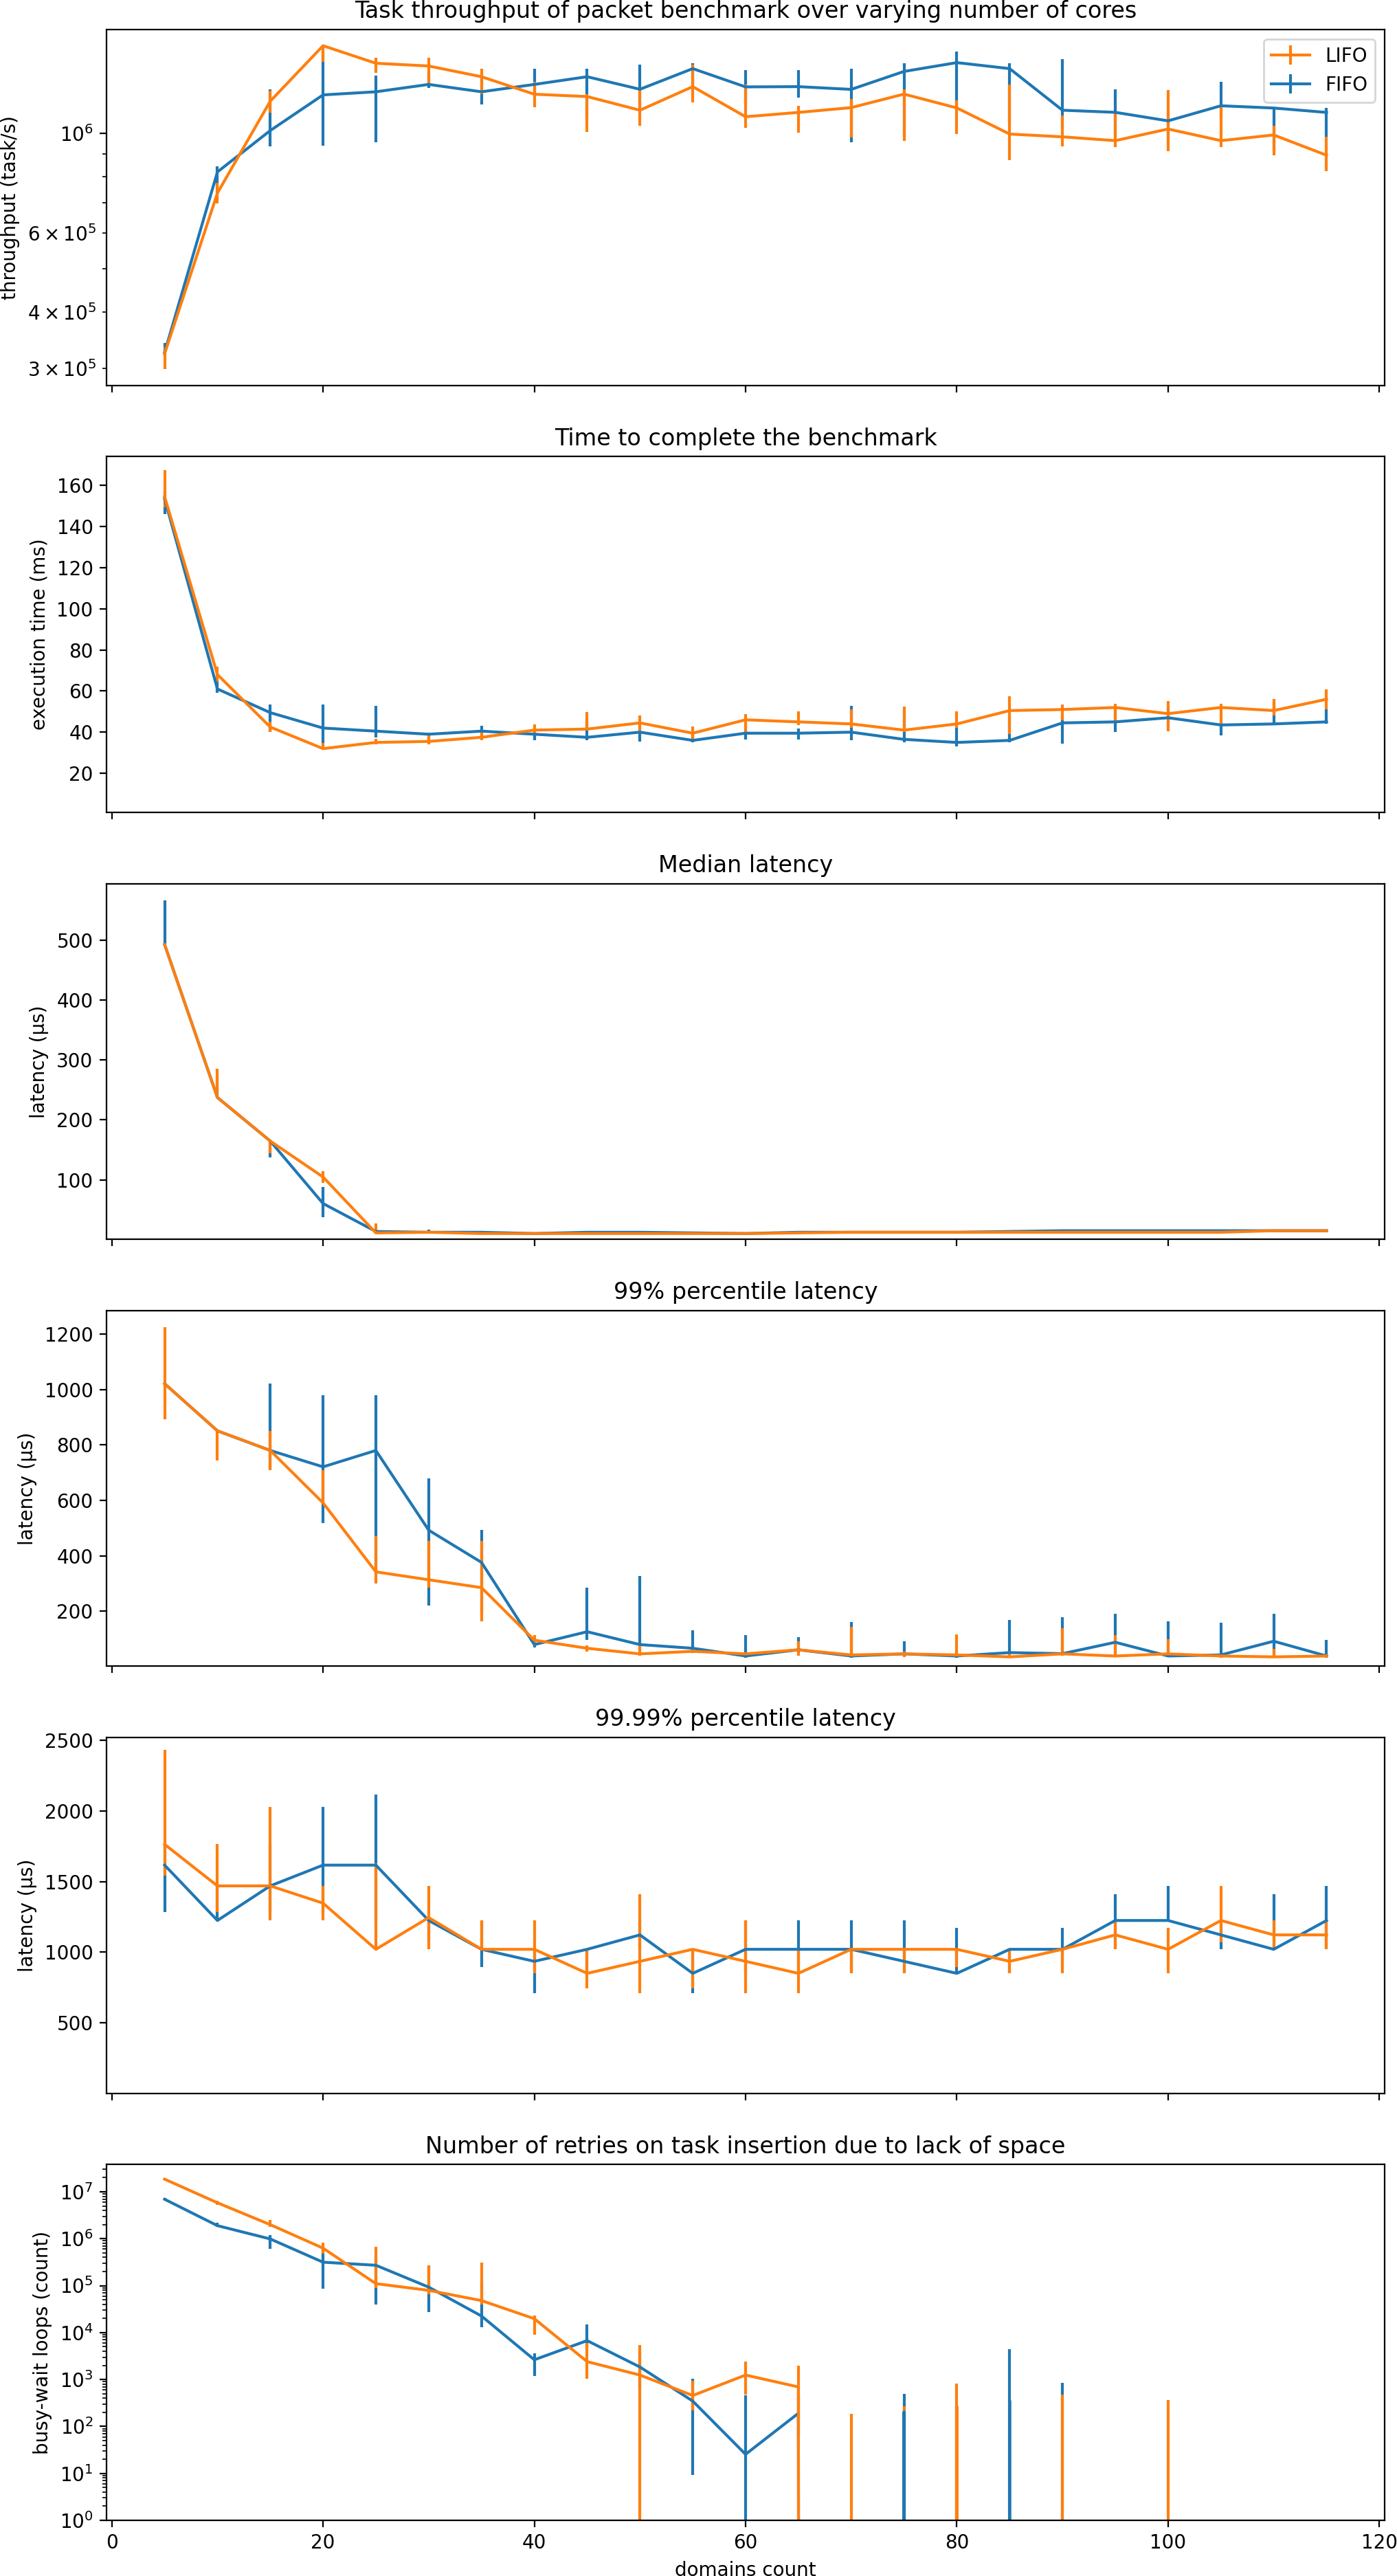
\includegraphics[width=0.85\textwidth]{eval/packet-basic-with-steal-counts2std.png}
     \caption{50k.}
    \label{fig:packet-50k}
\end{figure}

The first benchmark mimics a minimal TCP packet processing scenario. The workload relies on a single spawner as it would be the case with a server listening on IP and port tuple. To minimise the noise, actual network is not used. Instead, the \textit{server} thread chooses one out of 10 pre-made packets, copies it and schedules a handler task by performing an appropriate effect. The benchmark focuses on max load scenario and spawns tasks as fast as only possible, until the requested total is reached. Then, it monitors an array of thread-local counters, which are increased by successfully terminating tasks. Notably, the packets are between 2 and 3 KiB, and the spawner thread focuses solely on task creation. Therefore, cache locality does not significantly affect the performance. Likewise, the performance advantage of LIFO stealing does not apply to stealing from the spawner, as spawner never removes elements from its local structure. Local structure sizes are held constant at 128 elements, which is enough to keep the spawner from waiting with such small tasks.

The results of conducting a test with 50k packets in such a controlled setting are show by figure \ref{fig:packet-50k}. The first panel shows mean processing speed on a logarithmic scale. In the first part of the graph, between 5 and 20 domains, the performance rapidly accelerates with increase in the number of threads. 20 domains witness peak performance by LIFO scheduler and as more threads are added, the performance degrades. At first slowly, then faster beyond 80 domains. FIFO scheduler sees its peak at 80 domains but its performance is also relatively stable between 20 and 80, with a pronounced drop afterwards. This is surprising; adding more resources may not translate to a significant improvement \cite{amdahl} but it should not be detrimental either. Discussed further in \S\ref{section:degradation}. 

The second panel shows actual time required to complete the benchmark. Next, the charts from three to five show 50\%, 99\% and 99.99\% latency percentiles. Again, up to 20 domains there is a steep decrease in all latencies. There are local differences around 20 domains, with FIFO offering a better median latency for one point and LIFO better tail latencies for 2-3 points. Afterwards, the results converge. The tail latencies are partly driven by LIFO simply being faster to process tasks but, likely, not as much as it looks since error bars indicate more noisy measurement than elsewhere. 

Finally, the last panel shows number of retries of the main spawner (\textit{listener}) when trying to insert elements into the queue or stack. The retry loop is cheap to execute. Clearly, for lower core counts the spawner frequently throttles adding tasks due to lack of space. However, the number of busy-waiting cycles lowers with extra cores, quickly reaching point where magnitudes are too small to affect overall performance. At last, it ceases to occur in the median case beyond 45 cores. 
 
Both FIFO and LIFO perform very similarly on all metrics and exhibit similar phenomenons. As hinted in the first paragraph, the workload is so simple that it does not let some of the individual advantages prevail. There are slight differences, i.e. LIFO peaks at 20 domains, while FIFO at 80. But their overall performances (throughput and latencies) in ranges 0-20, 20-80, 80-115 are comparable.  Overall, it shows that both implementation are fairly balanced and a good foundation for benchmarking more complicated workloads.

\subsubsection{Degradation}
\label{section:degradation}
In line with Amdahl's law \cite{amdahl}, it is expected that any application will stop being able to take advantage of more resources at some point. After all, scalability is something to explicitely design for and even then, may not always be possible. However, there is no justification for more workers actually causing harm to the performance. Such a characteristic is highly undesirable in such a foundational system as scheduler. However, why would it arise in such a battle-tested idea as work stealing? 

\begin{figure} 
     \centering
     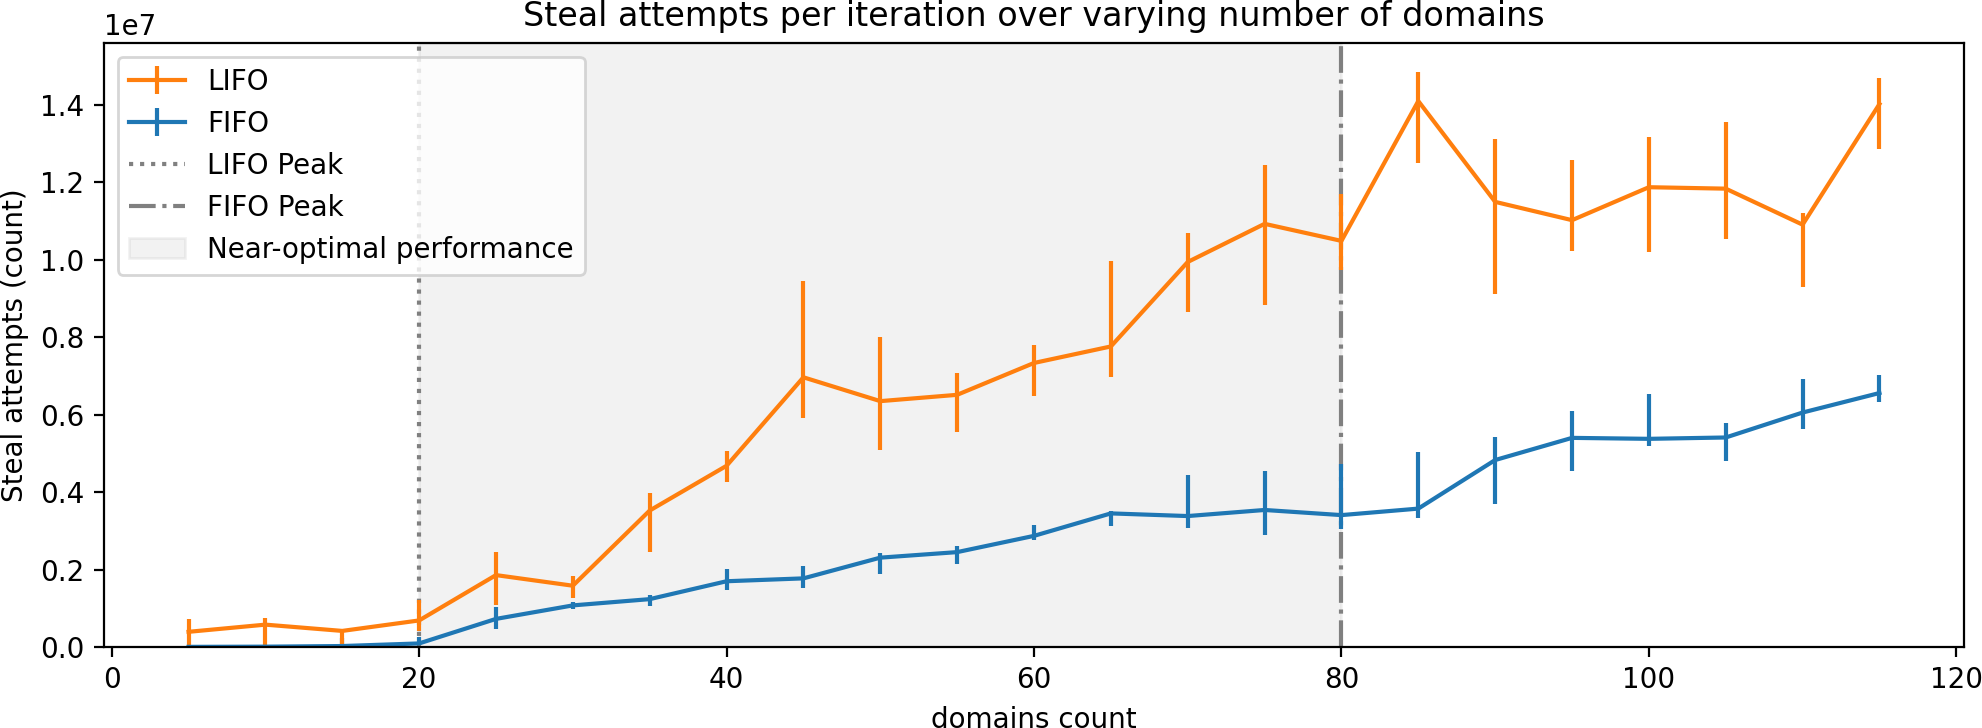
\includegraphics[width=0.85\textwidth]{eval/packet-basic-with-steal-counts2.png}
     \caption{The throughput achieved on 50k tasks over varying number of domains.}
    \label{fig:packet-with-steal-counts}
\end{figure}

In the LIFO case, as shown by \ref{fig:packet-with-steal-counts}, the scheduler is unable to maintain the increase in stealing attempts. Such increase is necessary for scalability, as each worker will need more stealing attempts to find the tasks. For example, if 1 out of 2 threads is spawning, the other thread has 100\% hit rate. On the other hand, if it is 1 out of 10 threads, then there are are likely going to be some misses or inefficiencies (minimal amount of work acquired). The diagram shows, that above 80 domains, as the information becomes more dispersed, the scheduler does not increase stealing attempts. In theory, there should be no scalability issues since each new worker also adds a new queue but in practise contention increases significantly as starved cores keep retrying and impeding the actual useful attempts. Conversely, if there is significantly more work and more time, the tasks saturate the system enough to prevent excessive stealing and observed negative effect ceases to exist (\ref{fig:packet-10m-throughput}).

\begin{figure} 
     \centering 
     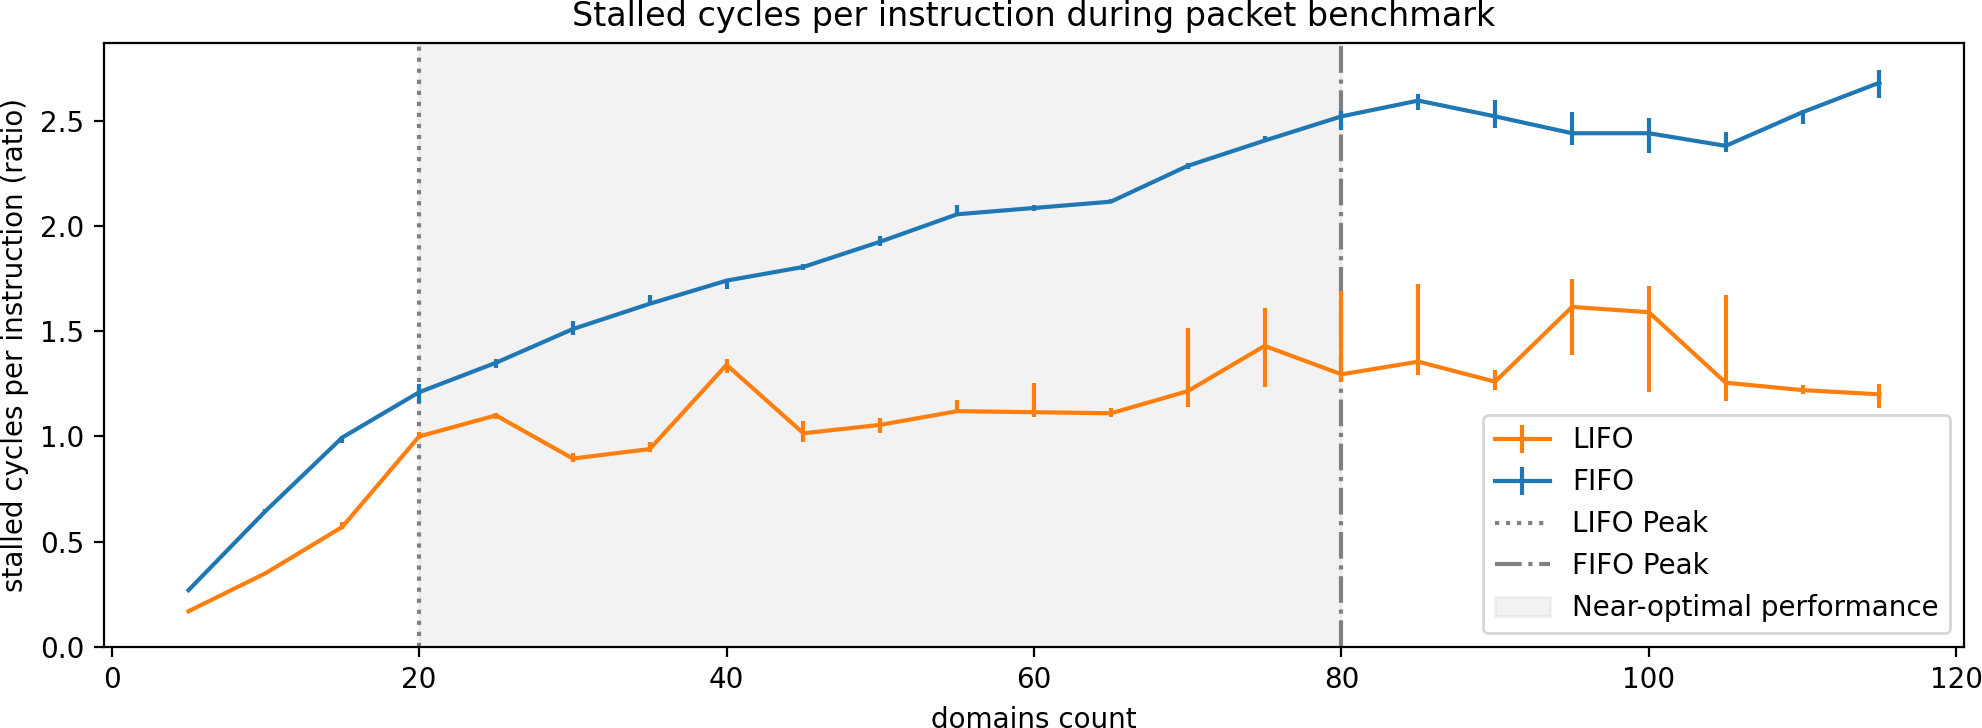
\includegraphics[width=0.85\textwidth]{eval/packet-basic-counters.png}
     \caption{The throughput achieved on 50k tasks over varying number of domains.}
    \label{fig:packet-counters}
\end{figure}

In the FIFO case, the problem also relates to work distribution. FIFO is not able to steal as much as LIFO because all steals compete with local dequeues, and, by design, those steals tend to lose the race more often since local dequeue uses a FAD rather than CAS to increment the index (\S\ref{section:wss-queue}). Therefore, while stealing alone is not maxed out, it significantly affects the rest of the logic. As shown by figure \ref{fig:packet-counters}, FIFO reaches over 2.5 stalls per instruction beyond 80 domains and this number keeps raising. The effect is also visible for LIFO but its pressure on the entire caching subsystem is much subtler.

Finally, it is worth stating that this result should not be interpreted as work stealing being generally inappropriate for saturating 100 cores. Packet benchmark creates a short burst of 50k items, which reaches a throughput of over 1.5m items per second. Each task has its own logic and requires allocations but it does constitute a very fine-grained concurrency. That puts a high pressure on the scheduler and exposes its inefficiencies. Further, there is an unusual amount of distribution required. It is far easier to distribute tasks onto 10 threads than 100 due to e.g. atomic operations taking constant time and load information is being less dispersed. If the workload is simplified just a little, the scalability improves. 

\begin{figure} 
     \centering
     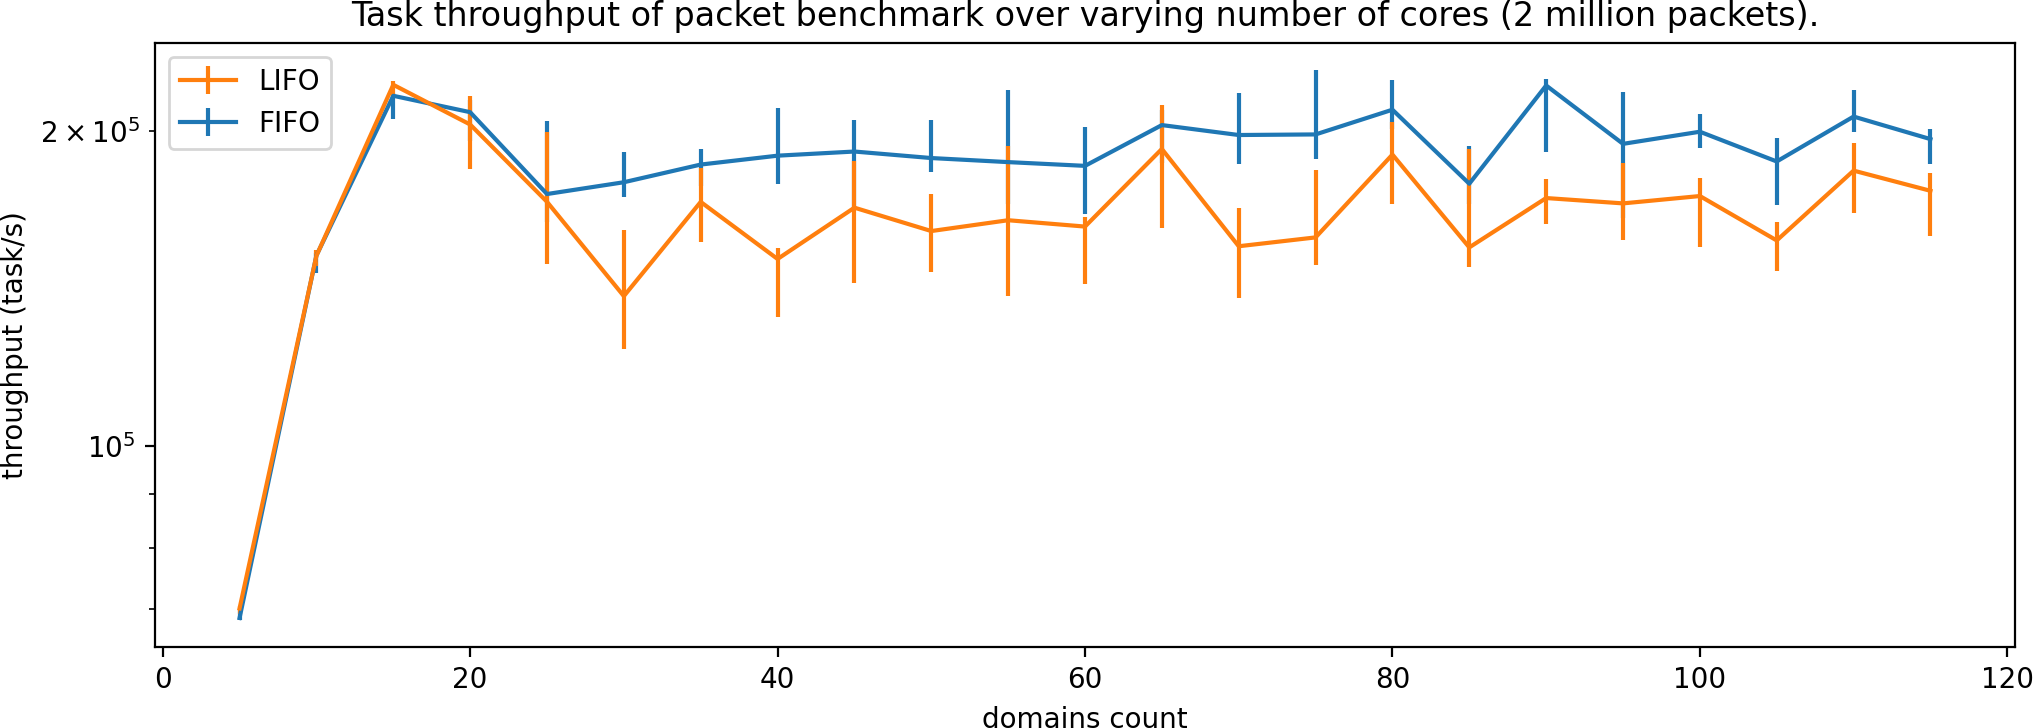
\includegraphics[width=0.85\textwidth]{eval/packet-basic-10million-just-throughput.png}
     \caption{The throughput achieved on 10 million tasks over varying number of domains.}
    \label{fig:packet-10m-throughput}
\end{figure}


\begin{figure} 
     \centering
     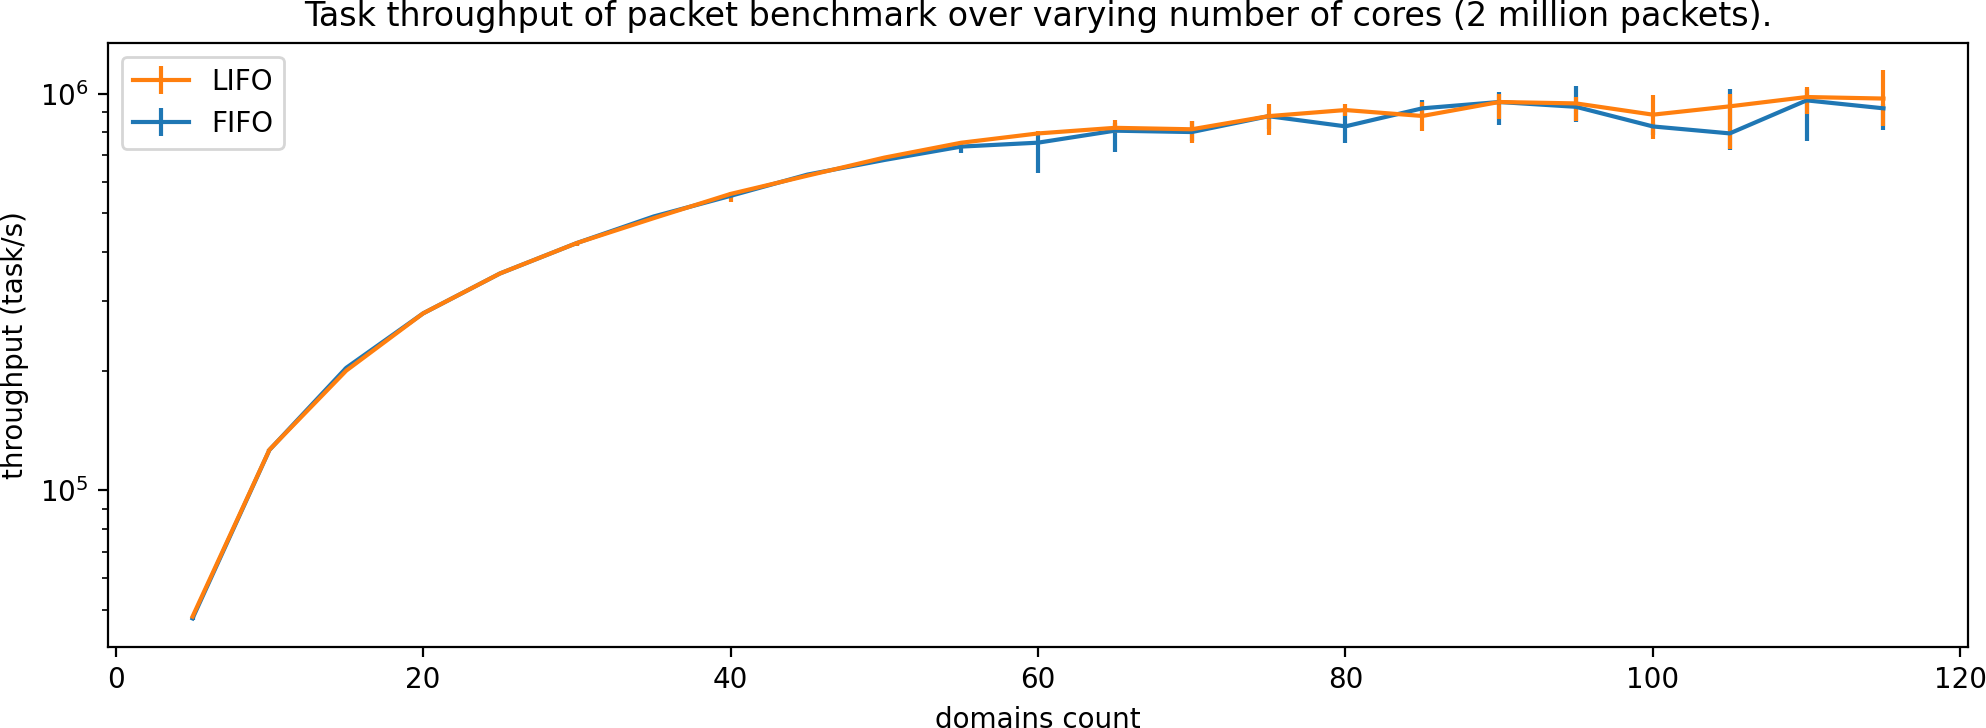
\includegraphics[width=0.85\textwidth]{eval/packet-basic-slowed_2.png}
     \caption{The throughput achieved on 50k tasks with over varying number of domains. Each tasks loaded with additional 500ns wait.}
    \label{fig:packet-slowed}
\end{figure}


\begin{figure} 
     \centering 
     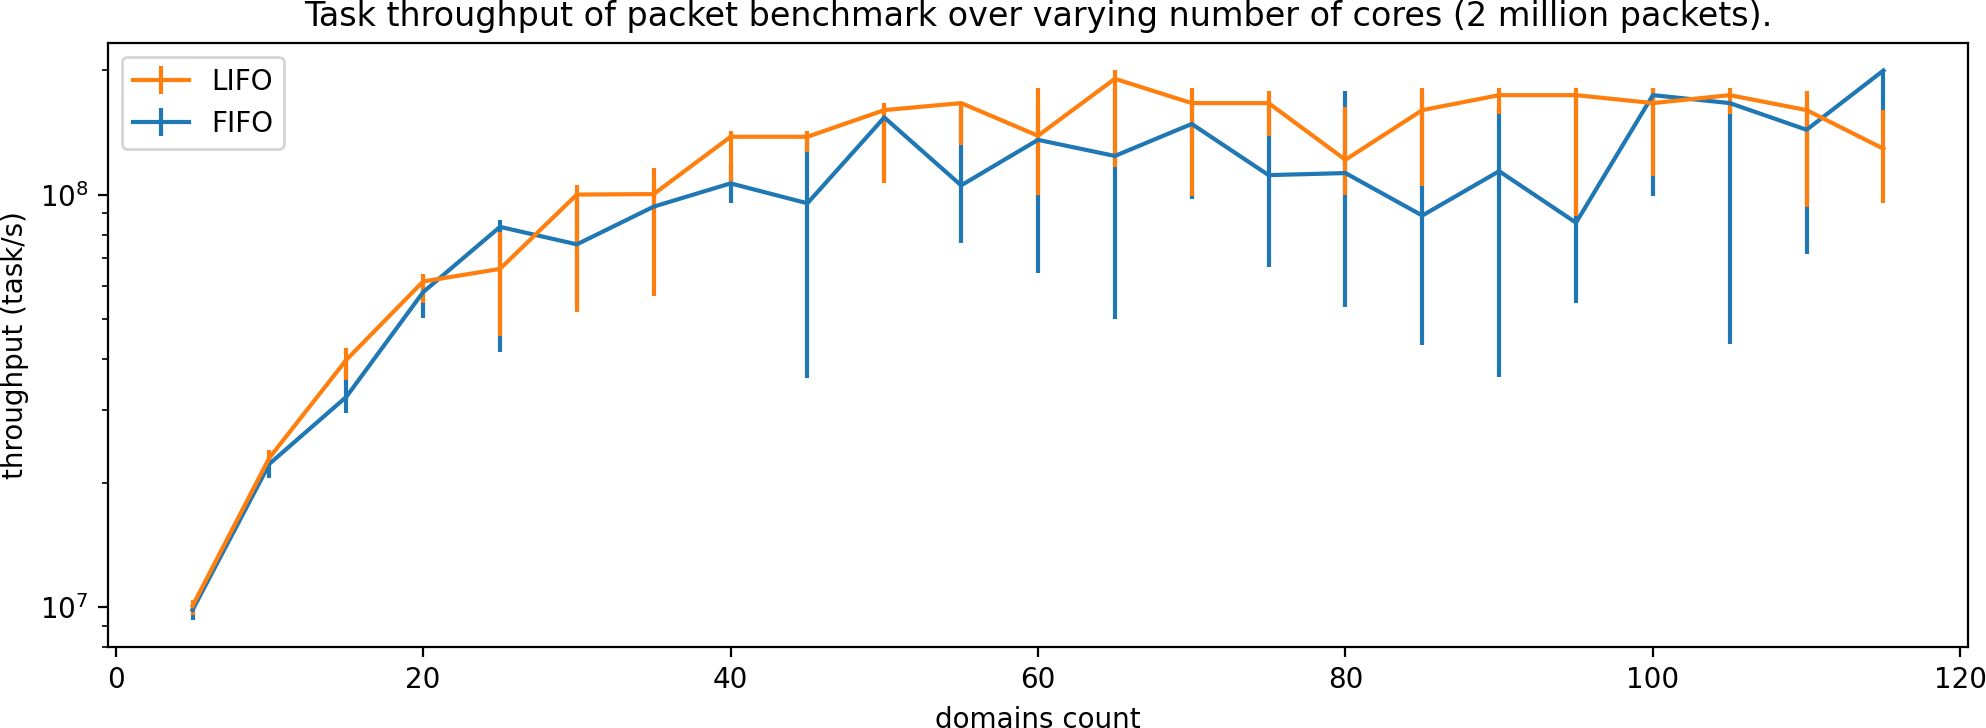
\includegraphics[width=0.85\textwidth]{eval/packet-basic-4spawners-just-throughput.png}
     \caption{The throughput achieved on 50k with 4 spawners. (2 spawners in the 5-core case.}
    \label{fig:packet-4spawners}
\end{figure}

\begin{itemize}
    \item \textbf{Heavier task}. See figure \ref{fig:packet-slowed} for the performance when each task has had an extra 500ns sleep to perform. This is enough time to extend the stability beyond 100 domains.
    \item \textbf{More spawners}. See figure \ref{fig:packet-4spawners} for the performance under more spawners, i.e. developer made an explicit change to help the scheduler.
    \item \textbf{Higher workload}. In fact, increasing the number of tasks also stabilizes the scaling. See figure \ref{fig:packet-10m-throughput} for the case with 10 million task instead of 50k. This case saturates many more workers, and while overall throughput is lower, the performance remains stable beyond 30 cores. 
\end{itemize}
These differences in scalability highlight the need for new methods to take advantage of high parallelism and very fine-grained concurrency (\S\ref{section:thesis}).


\todo{maybe there is a way to amalgamate these two?}
\subsubsection{Work Distribution Extensions}
\label{section:work-distribution-extensions}

Work stealing is robust but not perfect, e.g. the scalability ceiling describes in the \S\ref{section:degradation} or blind victim selection. As described in \S\ref{section:work-distribution}, regardles of primary work distribution mechanism, some sort of work stealing is necessary to prevent starvation in non-preemptive design with local structure. Otherwise, with a purely cooperative scheduling, any long tasks is going to significantly increase latency of all awaiting items. Therefore, a number of extensions to the core work stealing have been considered. They are motivated by the following observations.

\begin{itemize}
    \item \textbf{Contention.} The scalability of atomic operations and inter-processor communication is limited. Therefore, the design of stealing should be wary of those budgets as additional threads are added. 
    \item \textbf{Misplanning.} It might not make sense to steal a small number of tasks. If victim does not have enough work, the thief should simply look for another victim rather than conduct a steal and cause the victim to have to steal soon in effect. This could lead to starvation on blocking, thus the implementation simply has a bias to steal small number of items rarely. 
    \item \textbf{Blindness.} Random exploration of other threads local structures is inefficient. It causes contention and suboptimal steals. Instead, busiest threads should request help. 
\end{itemize}


The aforementioned observations translated into the following implementations. 

\begin{itemize}
    \item Reduce the contention on critical threads by having each thread only target its \textit{n} nearest neighbours in threads array. That creates a hierarchy along which tasks move and prevents the underloaded threads at the bottom of hierarchy from contending in the hotspots. Implemented with nearest 15 and 20 threads.
    \item \textbf{Steal at least 10.} Do not steal less than 10 elements as they will be efficiently processed by owner. Instead, look for work elsewhere. 
    \item \textbf{Work-shedding}. A polar opposite of work stealing. Busy worker randomly chooses another thread, which is forced to steal some of the busy thread's load. Notably, \cite{workshed} found improvement of tail latency stemming from extending work-stealing with work-shedding on a 32-core machine. Implemented as non-sticky, only a single steal is forced, and sticky, in which the victim keeps the target until another thread overrides it. 
    \item \textbf{Work-sharing from busy to free}. Requestor publishes its id in a highly-scalable lock-free queue. Threads looking for work picks up the id from the queue and steals work. This has the benefit of closing the information gap of pure work stealing or work-shedding. Only the overloaded and underloaded threads participate, while others remain unaffected.
    \item \textbf{Overflow queues}. Use extra structure for work distribution and put some tasks into a global queue. Here, spawner thread has a chance of inserting a tasks into global structure. Both Tokio \cite{Makingth53:online} and Go \cite{goprocgo14:online} feature global, locked queues for any tasks overflowing local queue. Three queues have been implemented: locked, lock-free, lock-free, 5-multi-queue. 
    \item \textbf{Local resizing}. Stealers aims to take half of its victims tasks. Increasing the size of local structure and the number of awaiting itmes may in turn lead to higher number of items distributed per steal. 
\end{itemize}



\subsubsection{Work Distribution Extensions Result} 
\label{section:extensions_result}

\begin{figure} 
     \centering
     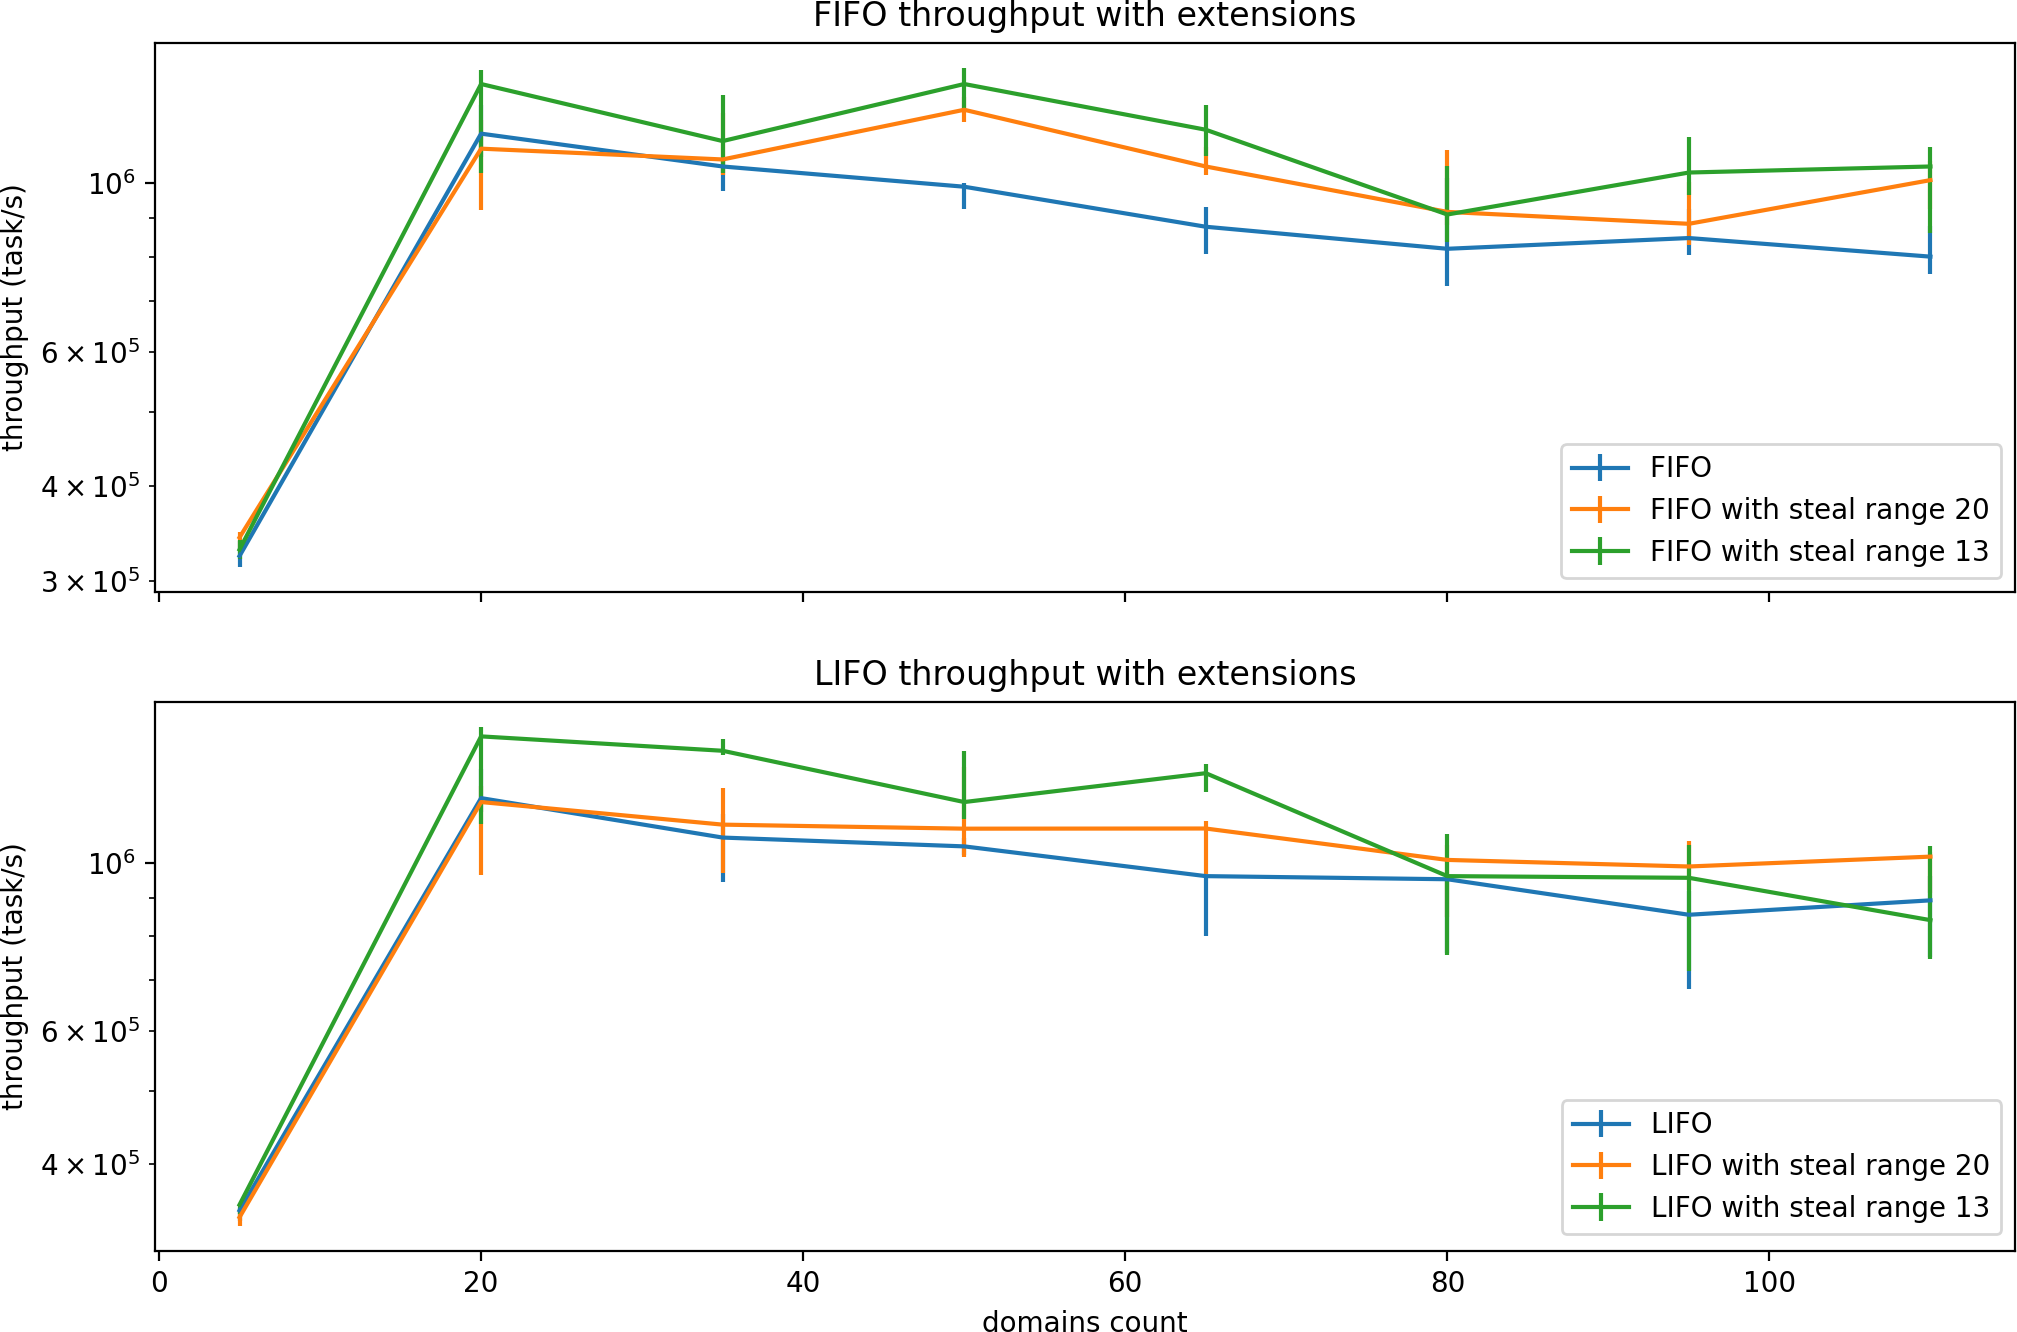
\includegraphics[width=0.85\textwidth]{eval/packet-basic-distribution10-granular.png}
     \caption{The throughput achieved on 50k tasks with over varying number of domains. Each tasks loaded with additional 500ns wait.}
    \label{fig:packet-extenstions}
\end{figure}


\S\ref{section:work-distribution-extensions} discussed a number of alternative work distribution mechanisms. The positive results are shown in figure \ref{fig:packet-extenstions}. Only neighbourhood stealing has shown a clear improvement over the baseline, which is in line with the diagnosis stated in the previous section \S\ref{section:degradation}. It is worth pointing out that such an optimization is going to have a negative effect on coarse-grained workload, where threads higher in the hierarchy are going to be stuck processing tasks for longer and thus not replenish its local structure quick enough. This result shows that very fine-grained workloads may require novel approaches and support the hypothesis (\S\ref{section:thesis}).

\label{paragraph:overflow-queue-bad-1}
Only stealing at least 10 elements had a strong negative effect, as it paradoxically increased the number of underloaded threads and contention on the loaded ones. Similarly, work-shedding approaches (sticky and non-sticky) resulted in other threads overloading the spawner and causing less efficient work distribution than random work-stealing. In pure work-stealing case tasks often flow through multiple hops, thus reducing the contention in the hotspot. The same effect was observed for simple locked overflow queues (as in Go and Rust) as the spawner has to compete with the workers for the lock.

Finally, scalable overflow structures (lock-free queue, multi-queue) and work-sharing from busy to free had an insignifcant positive effect. They would likely yield a stronger benefit for less heterogenous workload. Likewise, local resizing would be beneficial if starting size of the local structure was small enough.

\subsection{Server benchmark with cache effects}
\label{section:server-bench-with-cache-effects}

\begin{figure} 
    \centering 
    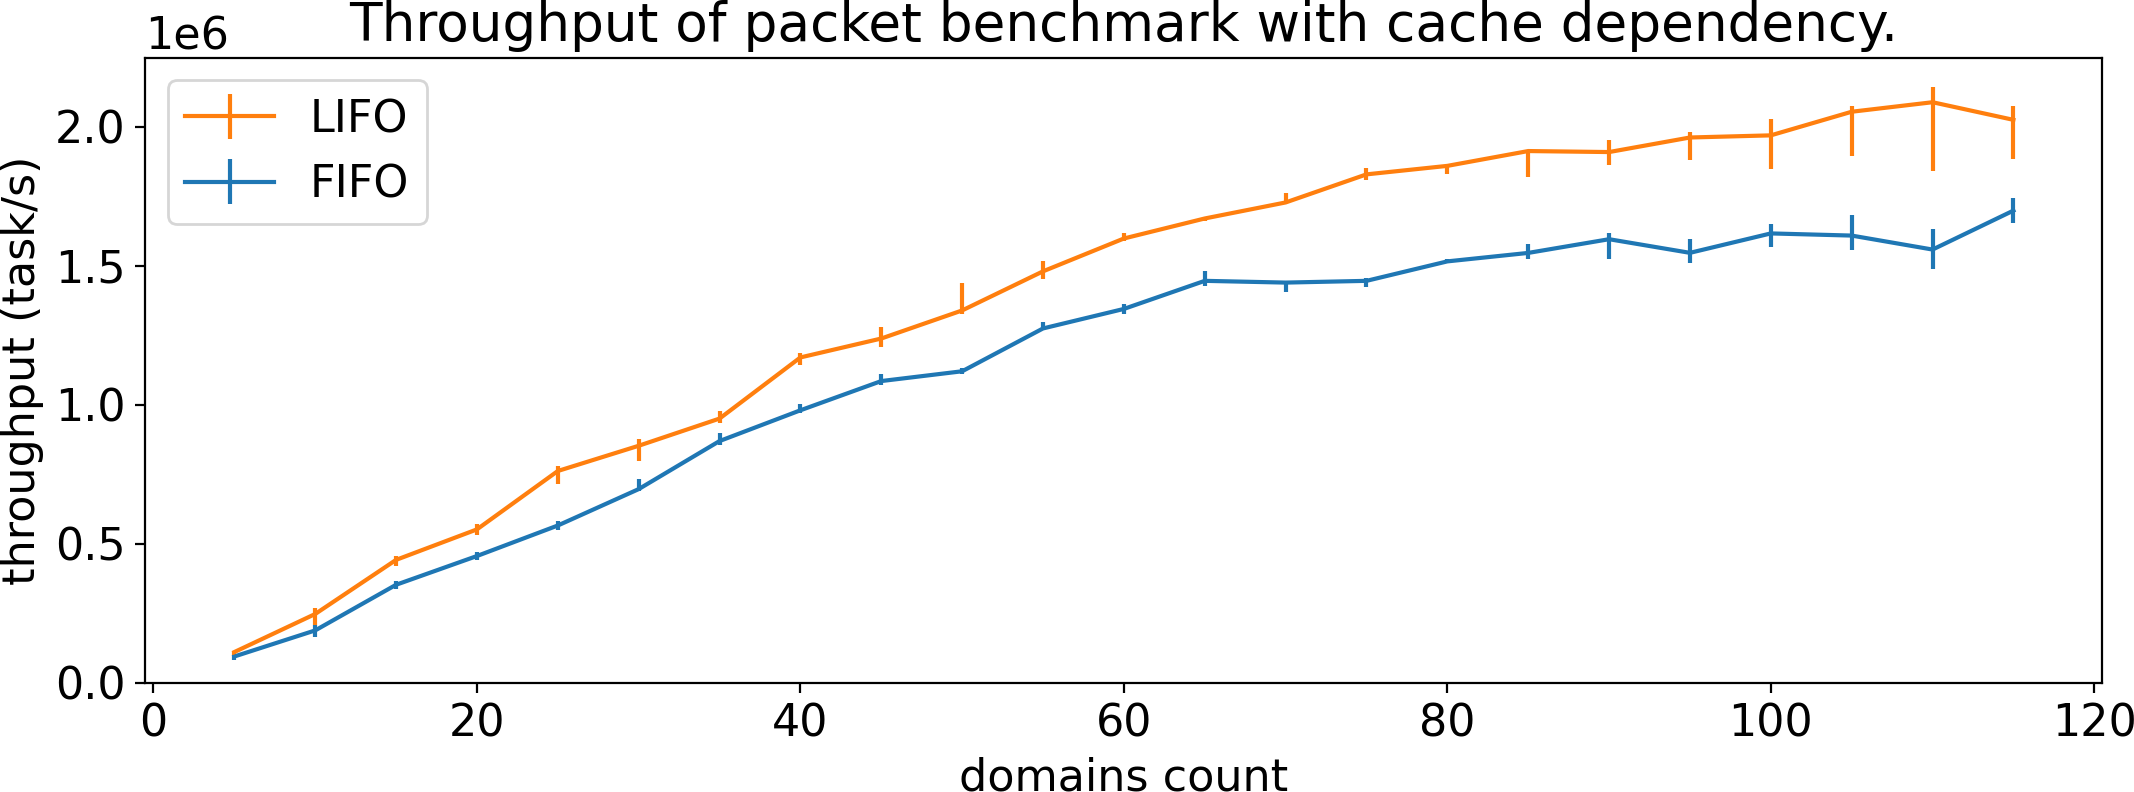
\includegraphics[width=0.85\textwidth]{eval/packet-basic-lifo-better.png}
    \caption{The throughput achieved on packet processing benchmark with 500k packets and 10 spawners. The benchmark was modified to have a non-trivial cache effect. Once the task was processed as in the original benchmark, it would spawn a chain of 10 tasks. Each task reads 20 with each reading 20 random bytes from the packet buffer, what simulates picking out different parts of the received data at different stages. LIFO offers a very clear throughput advantage (shown in the figure) and median-tail latency improvement.}
   \label{fig:packet-lifo-better}
\end{figure}

This section presents results of a more complicated workload, wherein once the packet is parsed, its contents are passed to the business logic. Namely, each packet from the general case benchmark (\S\ref{section:benchmark-general-case}) also spawns a 10-sequence of consecutive tasks. Each reads 20 random locations in the packet or does a simple computation (checksum), and spawns its child. That's until the depth of 10 is reached. Moreover, there are 5 spawners instead of 1, and individual queue sizes have been increased to 1024 to accommodate that. The results are shown by figure \ref{fig:packet-lifo-better}. Such a workload naturally favours LIFO, which can make a much better use of hierarchical memory and reduce cache misses. Thus, achieved throughput is far superior with LIFO ordering. Further, in line with the mechanics described in \S\ref{section:fairness-revisited}, using LIFO also significantly improves tail latencies.

Notably, extra care is required to replicate this result on modern architecture. For example, simple iteration over the packet in consecutive task does not experience memory inefficiencies due automatic memory prefetching. After a few first cache fails, the rest of the packet is going to be loaded into cache preemptively. This effect breaks down with any more complex memory patterns, which microarchitecture cannot predict.   

\subsection{Server benchmark with multi-modal processing latency}
\label{section:server-bench-with-multi-modal}

\begin{figure} 
    \centering 
    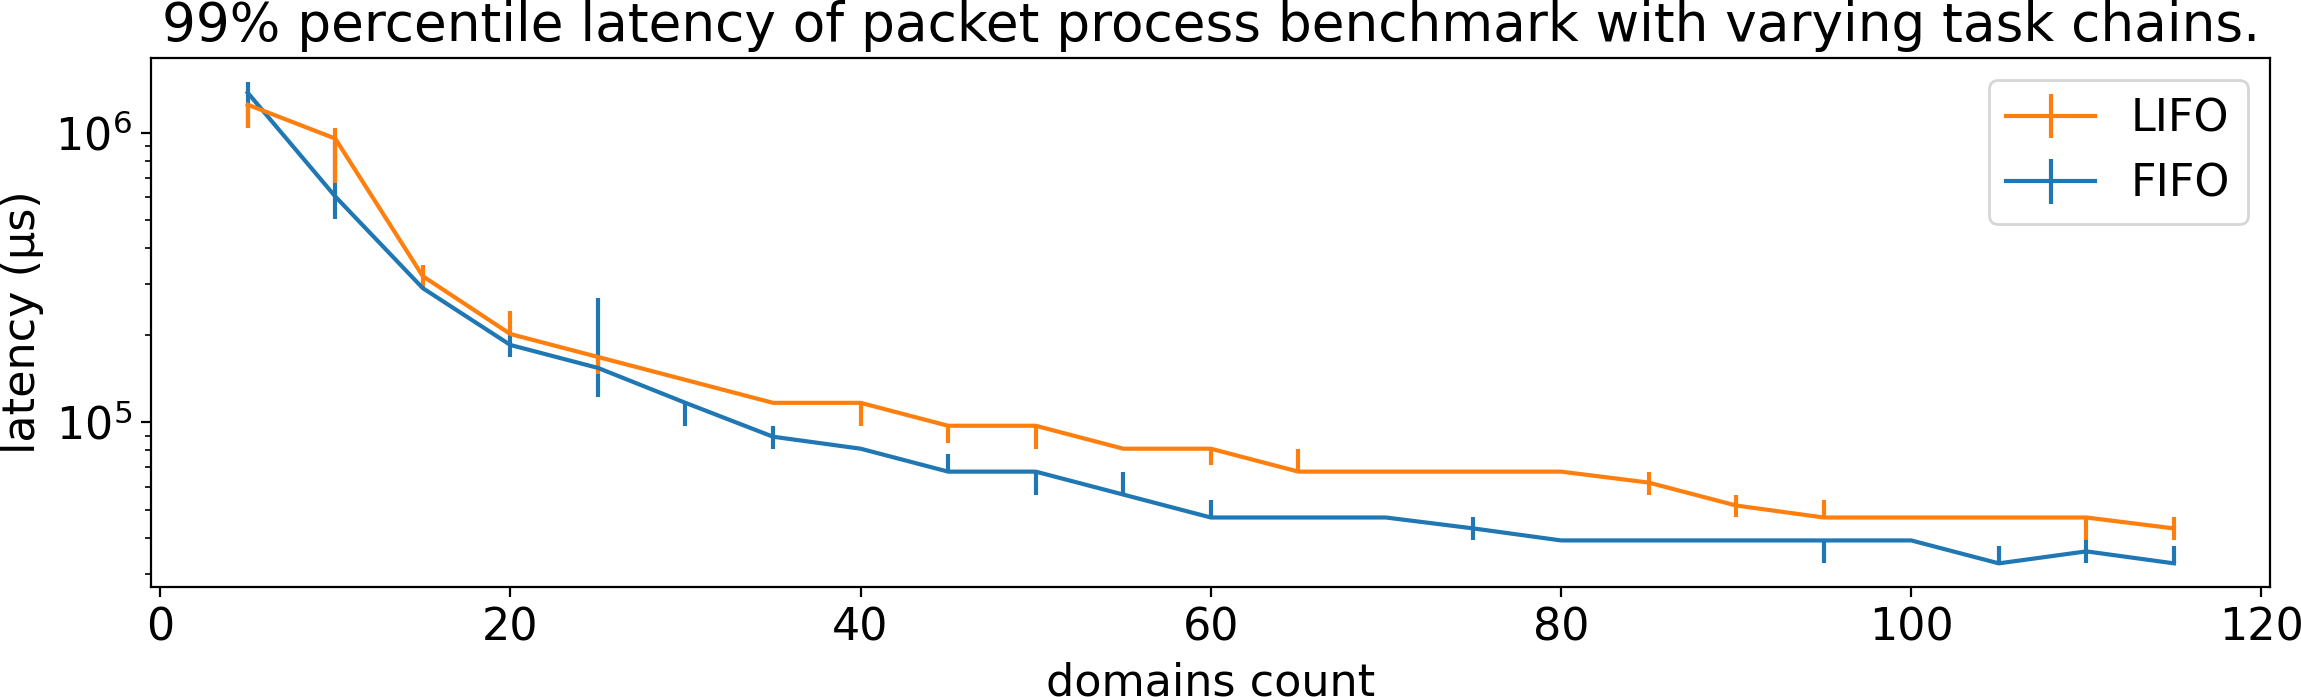
\includegraphics[width=0.85\textwidth]{eval/packet-basic-fifo-better.png}
    \caption{The throughput achieved on packet processing benchmark with 100k packets and 10 spawners. The benchmark has a weaker cache effect than \ref{fig:packet-lifo-better} but still significant enough for LIFO to have a better throughput. However, there is a 0.1\% chance that packet causes heavy work to be done, which spawns two tasks taking 20ms to complete. Akin to a network call to a different service. As shown in the figure, FIFO clearly offers a much better tail latency for most domain-counts in such a scenario. For example, at 115 domains LIFO saves over 30\% of tail latency.}
   \label{fig:packet-fifo-better}
\end{figure}

Figure \ref{fig:packet-fifo-better} shows results of a different twist to the packet benchmark than previous section. Here, instead of 10-sequence, only 3-sequence is spawned and the last task has a 0.1\% chance to spawn another task with lengthy operation. The 3-sequence still has cache-dependcies, which favour LIFO, but optional final task sets a trap. If scheduler processes the lengthy operations without care, it risks massively increasing latency of awaiting tasks. This favours FIFO, which is able to process lightweight sequences concurrenctly with the heavy ones, and have the lightweight tasks terminate early. The heavy operations wait longer but in their case the processing time is big enough for extra waiting to have a marginal impact. 


\subsubsection{LIFO heuristics}
\label{section:lifo-heuristics}

Pure LIFO scheduling is prone to poor tail latencies. Therefore, a number of heuristic has been implemented. They aim to integrate FIFO and LIFO ordering in a way that improves upon both, or at least provides a new point in the trade-off space.
\begin{itemize}
    \item \textbf{Alternating}. LIFO and FIFO removal alternately. Simple combination of pro-latency and pro-locality choices. 
    \item \textbf{Random}. Just as alternating, but the ratio does not have to be 50:50. Instead, it has been tested as 80\% LIFO, 20 \% FIFO and vice versa.  
    \item \textbf{Temporary FIFO ordering}. To prevent any items from lingering at the bottom of the stack, every 256 items, do as many FIFO removals as was the number of elements in the stack. Such approach is commonly known as reversing the stack but this implementation avoids the edge case of an item getting stuck between two infinitely deep tasks.
    \item \textbf{LIFO slot}. Rely on FIFO ordering but have a special slot for the most recently scheduled task. When looking for work, check this slot first. This violates FIFO and helps preserve locality between a chain of tasks. Featured in real-world projects, e.g. \ref{section:rel-work-go}. 
\end{itemize}
Notably, these heuristic have been built as a wrapper around LIFO data structure but have no direct support. Thus, by design, they are costlier to use. 

\begin{figure} 
    \centering 
    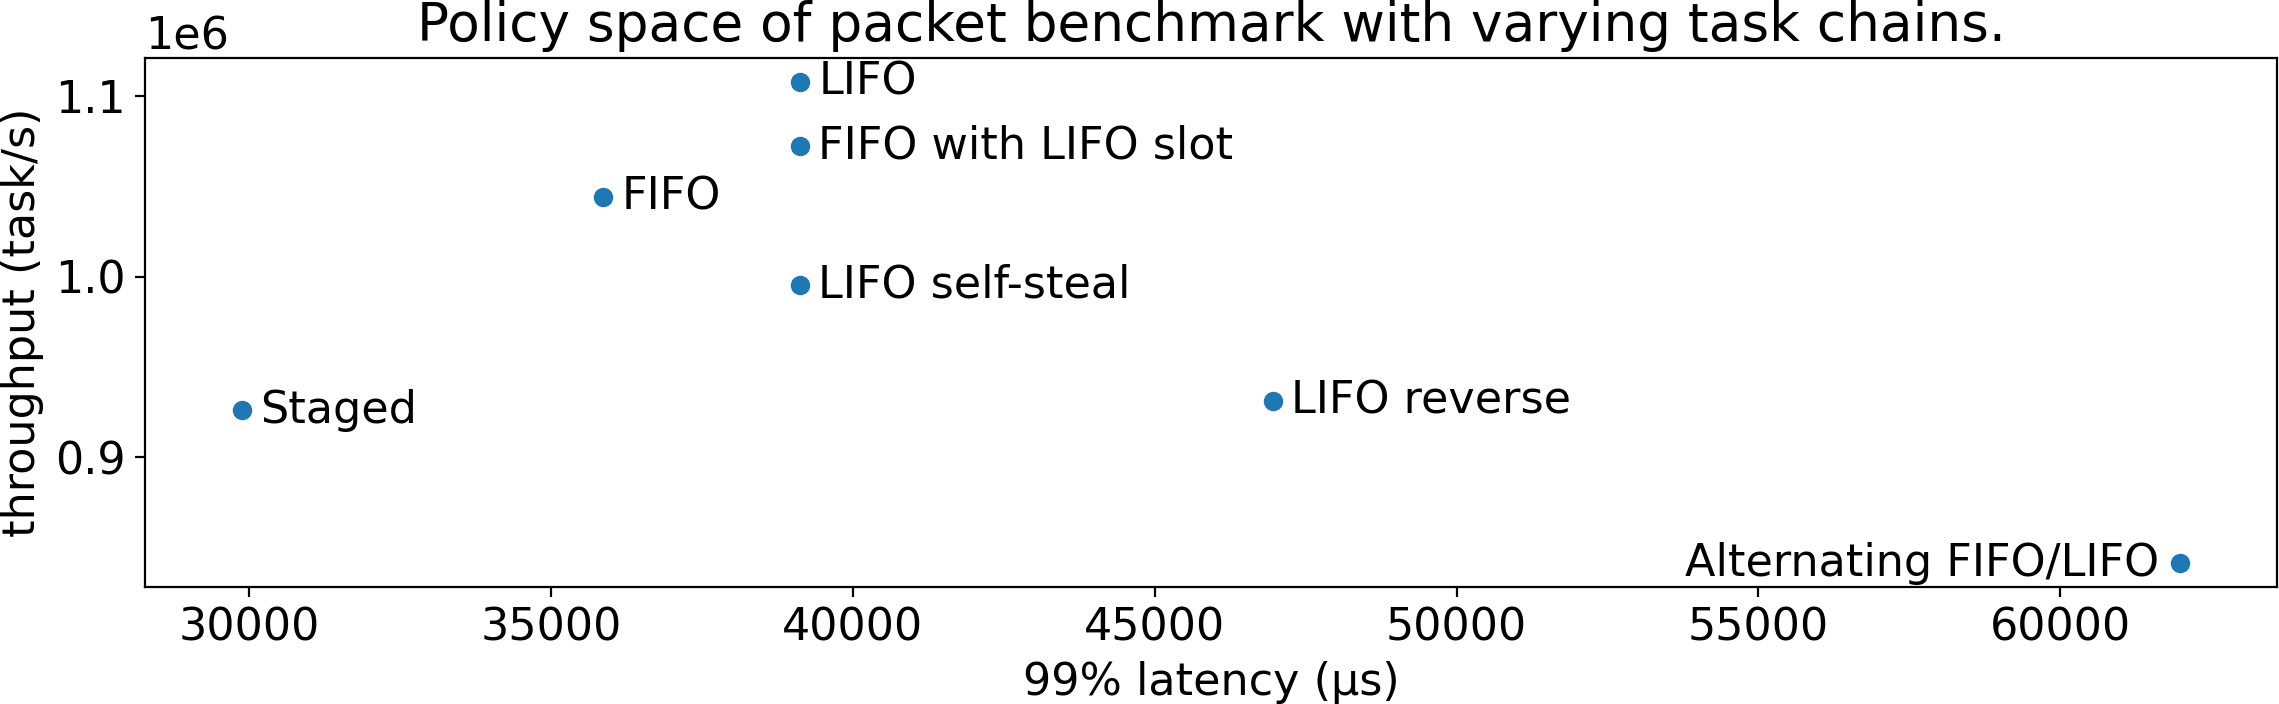
\includegraphics[width=0.85\textwidth]{eval/packet-basic-base-hybrids.png}
    \caption{The throughput and latency trade-off space achieved by various schedulers on the packet processing benchmark with varied task chains. The frontier consists of pure LIFO, FIFO and staged architecture, whereas various hybrid heuristic offered no benefits.}
   \label{fig:packet-hybrids}
\end{figure}

The baseline approaches described in \S\ref{section:impl-schedulers} and a number of heuristics decribed above have been tested. See figure \ref{fig:packet-hybrids}. Staged architecture was the only one to offer a useful point in the trade-off space, in the form of significantly superior tail latency at the cost of throughput. This gain stems from having a pool of threads dedicated directly to the lightweight tasks. The fall in throughput is difficult to avoid in a workload that work stealing is able to scale efficiently. Nonetheless, if the final task was lighter, it is possible for staged architecture to improve on both metrics, as observed with artifical benchmarks. 

This result, in line with hypothesis (\S\ref{section:thesis}), strongly support the benefits of customizing schedulers. Even for the same workload different policies may be appropriate depending whether throughput or latency is more important. In fact, just the fact of composing multiple baseline schedulers using queues significantly improved tail latency.

\section{Mixer benchmark}
\label{section:mixer-benchmark}

\begin{figure} 
    \centering 
    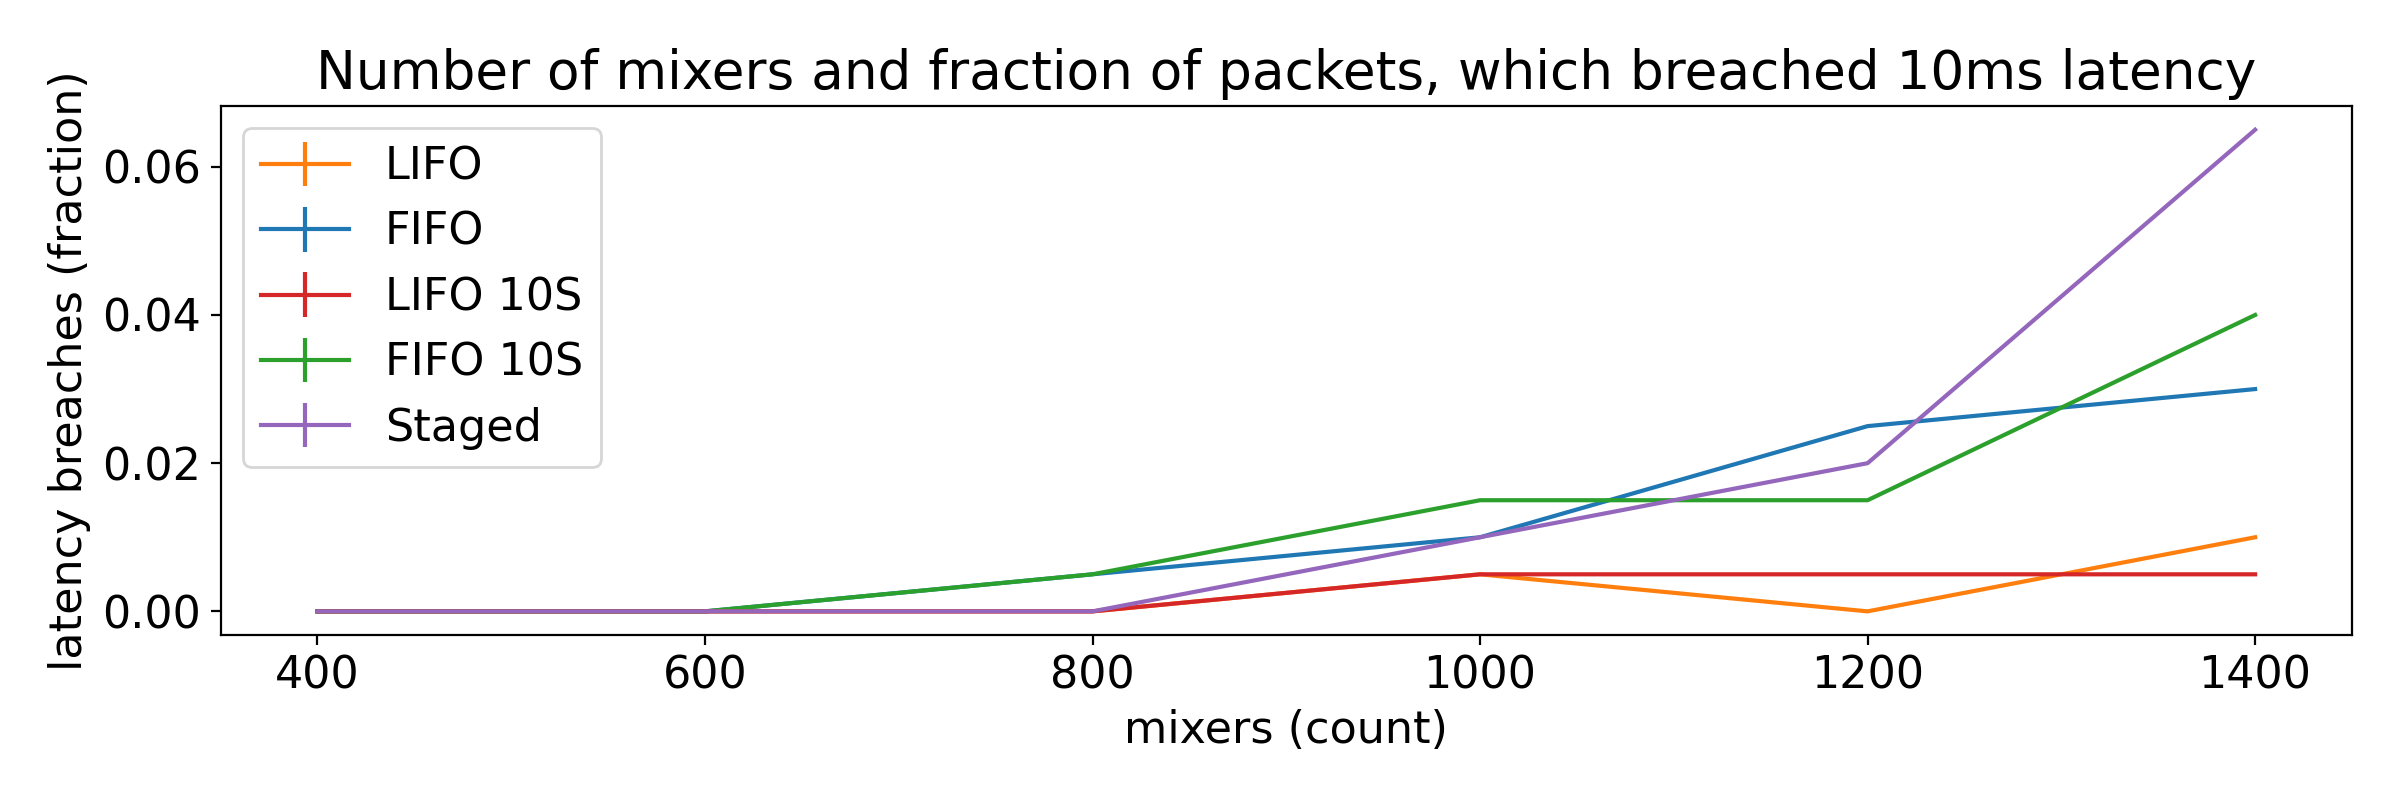
\includegraphics[width=0.85\textwidth]{eval/mixer-base8.png}
    \caption{The number of latency breaches achieved by different schedulers as the load (number of mixers) increases.}
   \label{fig:mixer-bench}
\end{figure}

The mixer benchmark represents a complicated real-world use case. It derives from architecture of a VoIP softswitch - FreeSWITCH (\cite{Maruzzelli2017-ou}), which heavily relies on threading. FreeSWITCH runs multiple OS threads for a single call. Firstly, there is a thread for the conference. It collects audio from all participants, mixes it (hence mixer), and passes the output to all participants. However, there is a number of things that needs to happen for every participant. At the minimum, each participant can have a different codec setting, thus the incoming audio has to be decompressed for mixing and outgoing audio has to be compressed before sending. In practise, there is a lot of other per-call-leg logic as well, e.g. signalling, jiter buffer. Therefore, there is also a single thread per participant. In such a setting, mixer thread only interacts with participant threads, which in turn interact with external world. 

Such a workload is particularly difficult to optimize for due to its complexity. It features short-lived and long-lived tasks. Some tasks benefit from cache locality, while others not. Many details will vary over time, e.g. distribution of number of people in mixers (as conference could have anywhere from 3 to hundreds people), length of calls, codec selection, media routes (IP-to-IP) \cite{Frequent1:online}, etc. Moreover, the workload makes heavy use of many high-level features such as yielding (\S\ref{section:yield}) and promises (\S\ref{section:promise}), which are not the typical targets of high-performance optimizations. Therefore, in this case, the robustness is just as important as overall performance. 
 
Crucially, participant and conference threads yield frequently. They simply cannot make progress witout data. Yielding threads have to be placed in an external global structure (\S\ref{section:yield}), here a multi queue. This seems suboptimal because locality is not respected, and centralization of tasks is rarely the desired state. Therefore, on top of FIFO, LIFO and Staged, one more approach has been evaluated. It is a composition of 10 individual schedulers (FIFO or LIFO) in order to silo particular sets of conferences and participant threads. This imposes boundaries on stealing and yielding since whatever happens the task remains in its silo. Akin, in spirit, to neighbourhood stealing (\S\ref{section:extensions_result}).

\label{paragraph:overflow-queue-bad-2}

Figure \ref{fig:mixer-bench} shows the ratio of latency breaches of different schedulers over increasing number of conferences. This metric behaves similar tail latencies. LIFO performs the best as it is able to capitalize on mixed down audio by immediately sending data back. FIFO sees significant number of fails early, what is explained by the (effectively) constant depth of task graph (\S\ref{section:fairness-revisited}). Staged is unable to capitalize on having multiple stages because even in the base FIFO and LIFO case, most of the scheduling goes through the global multiqueue. In such a case, Staged only has extra overheads and adds another queue before sending out mixed down audio, where it is not beneficial to prioritise other work. Curiously, siloed FIFO and LIFO did not differ significantly from core implementations. Locality benefits are not big enough to make a difference in this case. It is also a point of in favour of scalability of the base designs. Notably all schedulers have been fitted with highly-scalable multi-queue for overflow queue. A scheduler with lock-based overflow structure (as in the case of \S\ref{section:rel-work-go}, \S\ref{section:rel-work-rust}) does not terminate in reasonable time.

Finally, this result shows that even when optimizing for latency, there is no ready-made solutions. In the case of server benchmark with multi-modal packet processing latency (\S\ref{section:server-bench-with-multi-modal}), the best latency was offered by Staged architecture and the worst by LIFO. The mixer benchmark is exactly opposite: LIFO is the best choice for latency and Staged the worst. This phenomenon is another example of the hypothesis (\S\ref{section:thesis}). 

\section{Binomial option pricer benchmark}
\label{section:binomial_option_pricer_result}

\begin{figure} 
    \centering 
    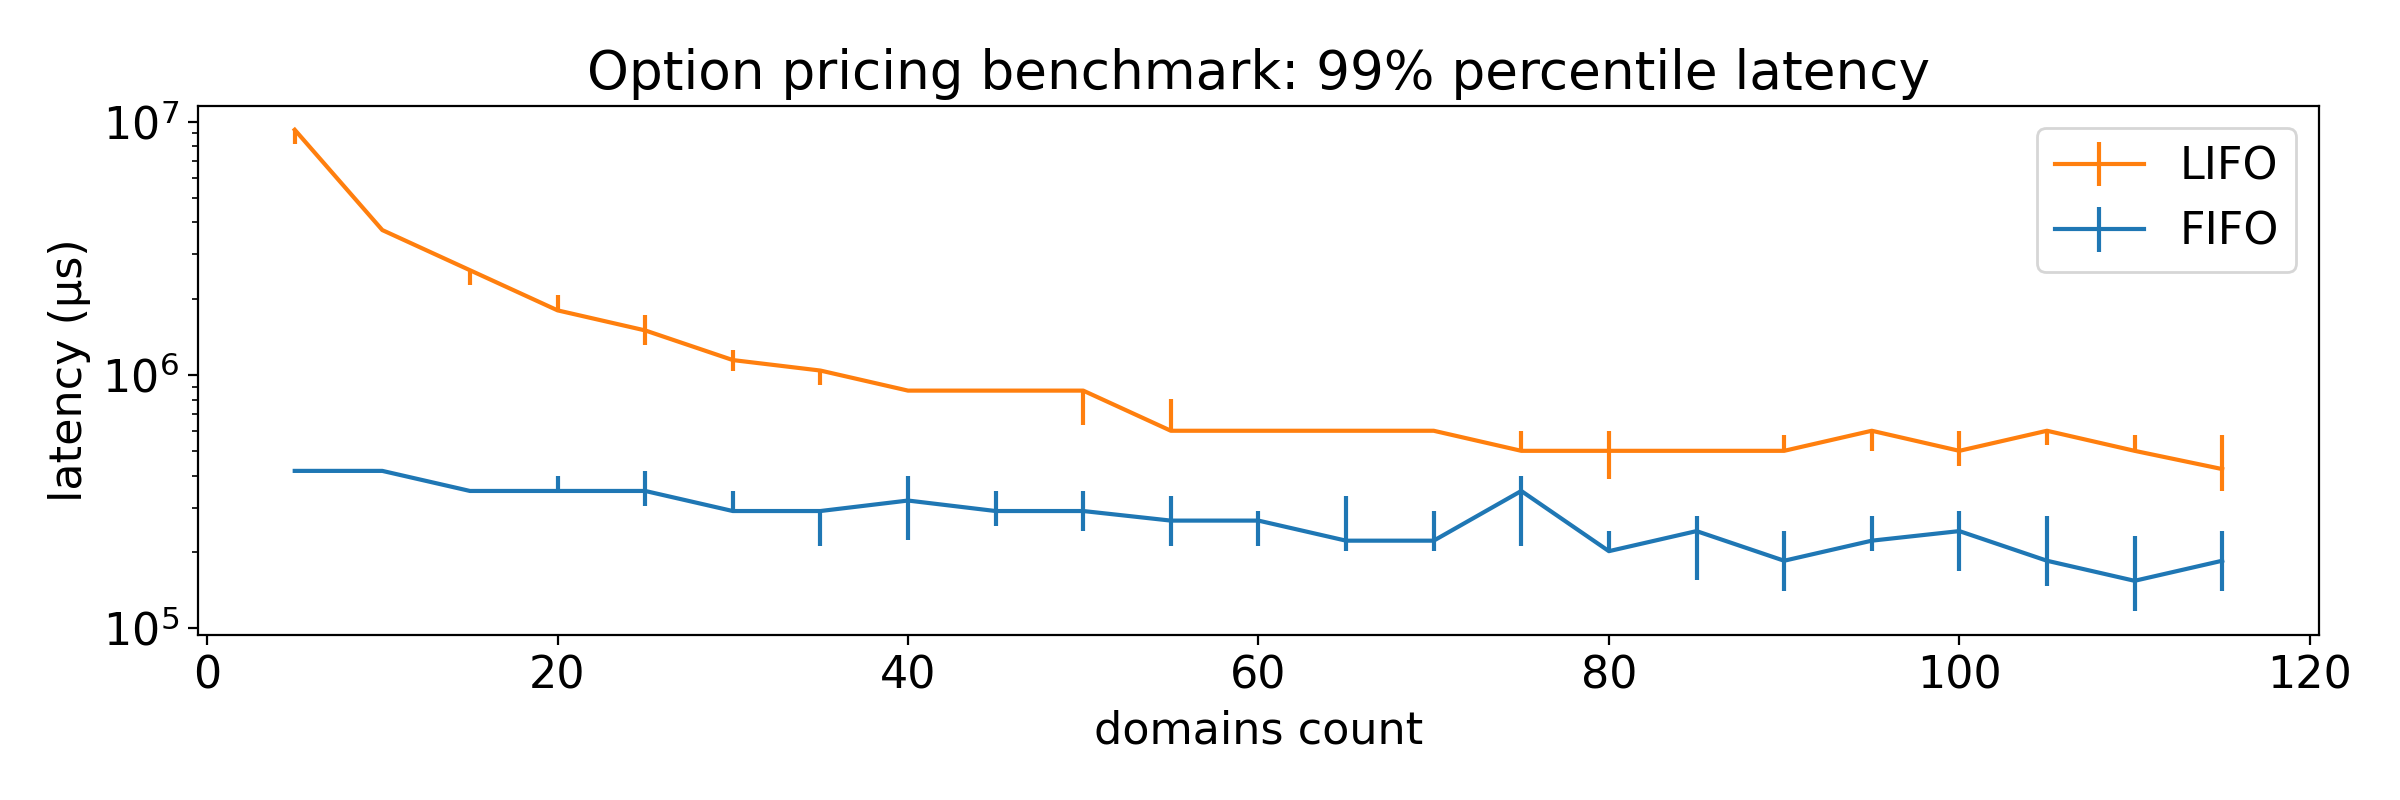
\includegraphics[width=0.85\textwidth]{eval/options-base.png}
    \caption{The number of latency breaches achieved by different schedulers as the load (number of mixers) increases.}
   \label{fig:options-bench}
\end{figure}

Option contracts are financial derivative instruments, which provide the holder with an option (but not an obligation) to enter a specific trade a some point in the future. For example, a european call option on Google with strike price of \$2600 and expiration date of 2022-03-06 lets the holder buy a specified number of Google shares at the strike price and on the expiration date \cite{Hull_John}. Value of an option at expiration depends strictly on the the price of its underlying.

\begin{center}
$call\:option\:value = max(underlying\:price - strike\:price, 0)$.
\end{center}

Binomial model first estimates value of the underlying by assuming that at each time step the price may either move up by a specific amount or down by the inverse, at specific probabilities. This creates a lattice, whose leaves represent prices at some final timestep. Then, the binomial pricer calculates payoff at every final timestep and propagates the expected value backwards using known probabilities of up and down moves. The first stage - stock prices at final timestep - can be computed analytically, while propagation of expectation must actually walk the lattice to take interest rates into account. Despite its simplicity, the binomial model is widely used in practise as it is far easier to include extra features than in the analytical approaches.

In constrast with other asset classes, computation of option prices is computationally intensive due to sheer number of instruments. For example, NYSE has 2400 stock listings. Each of them has hundreds of options at different strike prices, expiration dates and contract terms. Thus, the benchmark recomputes values of 30k options. Differents instruments have varying importance to a trading company due to the size of current position, available infrastructure, other models, etc. Thus, most instruments are computed at a fairly low accuracy (20 timesteps) and 0.5\% at high accuracy (2k steps), what results in a bimodal distribution of work per instrument. Pricing of each option is not parallelized but each timestep of the lattice is computed concurrently to avoid long stalls. 

\begin{itemize}
    \item Despite an overall comparable throughput the latenyc is much better with FIFO
    \item The latency improves because more workers mean that queues are overall shorter, which means fewer items are stuck behind heavy tasks. Moreover, there is more stealing and the stealing always takes the oldest elements. 
    \item Increasing the number of spawners is tragic for latency on LIFO as that leads to more tasks being processed locally and in a more LIFO manner. 
\end{itemize}

Figure \ref{fig:options-bench} shows the tail latency under FIFO and LIFO scheduling. Even though that the overall throughput is comparable, the latency is significantly better with LIFO. It follows from FIFO processing each task-tree concurrently and taking advantage of terminating the shallow ones early. This benchmark may seem specific and inconsequential to most workloads, yet this is what commonly occurs in complex systems. Distribution of tasks is not just bimodal but multimodal, and thus impact all range of tail latencies. In fact, in the limit, if some subtrees have infinite depth, other tasks may never get to run with LIFO. Practical runtime or systems schedulers typically follow FIFO to avoid starvation in heterogenous workloads.   

As more workers are added, the tail latency improves. Predominantly because the overall queue sizes are shorter (fewer items are stuck behind heavy tasks) and stealing always takes the oldest elements. However, as soon as more spawners are added, the spawning becomes more efficient and processing more local, what collapses the tail latency even with many domains. 

Notably, this results contrasts with the other complex benchmark (\S\ref{section:mixer-benchmark}), where LIFO scheduler is the way to optimize latency. Furthermore, in the previous cases (e.g. \S\ref{fig:packet-4spawners}) increasing the number of spawner improved both throughput and latency since it helped to loose the bottleneck in work distribution. In the case of options pricer benchmark, adding more spawner does improve throughput but hurts tail latency as queues grows and processing becomes more LIFO. Again, these phenomena show importance of customized scheduling (\S\ref{section:thesis}).

\section{Comparison with Domainslib}
\label{section:result_with_domainslib}

Note, the LIFO in this section refers to the LIFO scheduler developed for this project. Domainslib (which is also locally-LIFO) is referred to explicitely.

\begin{figure} 
    \centering 
    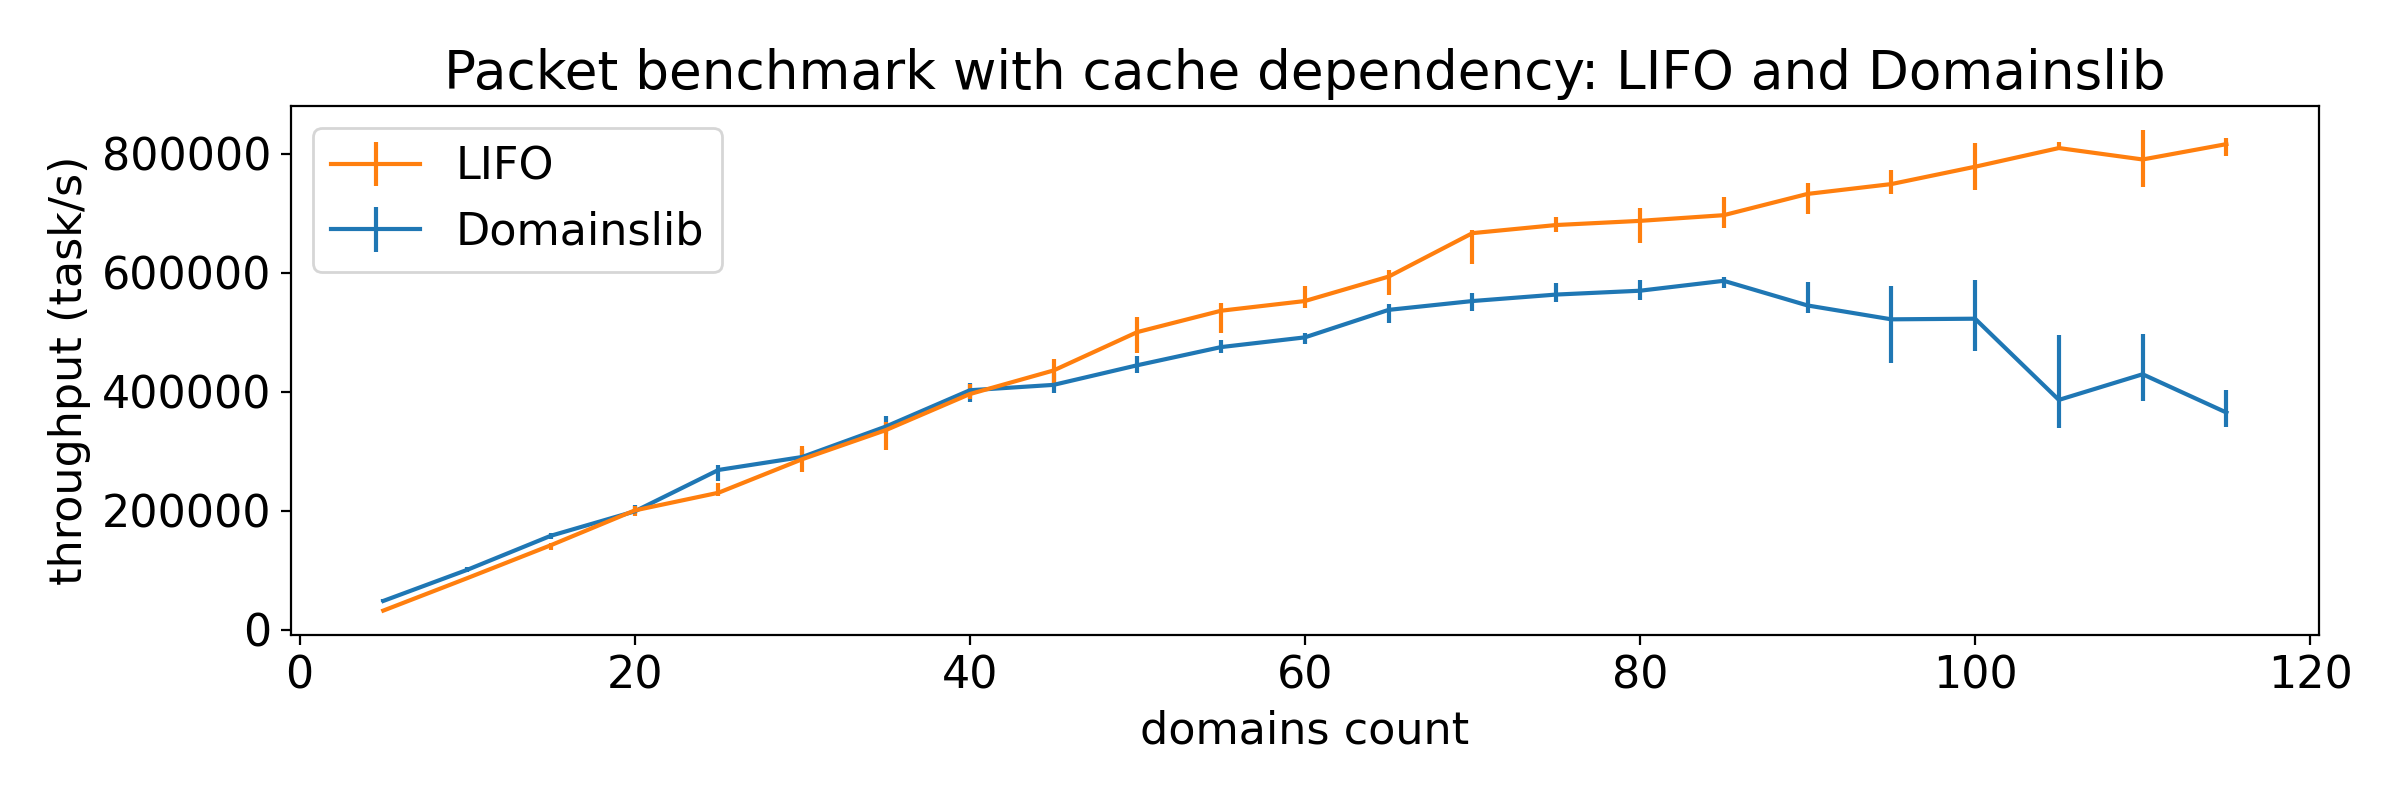
\includegraphics[width=0.85\textwidth]{eval/comp-base4.png}
    \caption{T 100k packets with cache dependency / just 1 spawner.}
   \label{fig:domainslib-comp}
\end{figure}

The performance with Domainslib has been compared using the last packet processing benchmark (\ref{section:server-bench-with-multi-modal}) as it features bimodal work distribution, cache effects and is assessed using a simple metric - throughput. Further, to highlight the effect, the benchmark was run with just 1 spawner. It is worth pointing out that Domainslib is able to auto-resize, while for LIFO, althought possible, auto-resizing has not been implemented. To account for that difference both Domainslib and LIFO were set to have a minimum size of 1024 items, which Domainslib can expand further if needed. 

The results are shown in figure \ref{fig:domainslib-comp}. The Domainslib is significantly faster at low core counts. Between 20 and 40 cores the benefit vanishes and both implementations offer a similar performance. Beyond 40 cores the Domainslib is unable to scale. It peaks at 85 cores and sees a very strong reduction in throughput for more cores. The LIFO implementation, on the other hand, sees diminishing results but continues to improve all the way to the last data point at 115 cores.  

The detailed analysis is beyond the scope of this section but the three key factors are described below.
\begin{itemize}
    \item \textbf{Optimization.} The constant factors of Domainslib are more optimized. It requires only a single atomic operation per insertion or removal. Moreover, Domainslib uses a number of advanced techniques that are possible to apply to the LIFO implementation, but are risky to use in the early development, e.g. \textit{Obj.magic}, forcing inlining, unsafe array operations. This aligns with figure \ref{fig:domainslib-comp} showing a constant improvement over LIFO in the 5-15 range. 
    \item \textbf{Scalability.} Domainslib only steals a single element at the time, while LIFO steals half of the items. LIFO only needs a single index operation per steal, thus the actual number of atomic operations per steal of both implementations converges as mor elements are stolen. But all Domainslib's atomic operations focus on the \textit{head} index. LIFO, on the other hand, in proportion uses the \textit{head} less and less. Furthermore, stealing multiple elements creates a load-balancing network, where elements propagate through multiple hops and ease stress on the spawner. With the steal-one policy, load on the spawner incrases linearly with the number of domains.
\end{itemize} 

\chapter{Summary and conclusions}

This dissertation focused on exploring the trade-offs between various real-world scheduling policies. The core of the work included lock-free FIFO and LIFO schedulers, which were then composed (\S\ref{section:staged-as-composition}) and extended in various ways (\S\ref{section:lifo-heuristics}, \S\ref{section:work-distribution-extensions}). The evaluation involved a number of real-world benchmarks and common industrial metrics: throughput and tail latency (\S\ref{section:objectives}). 

The results highlight vast differences between different scheduling policies. There is no single optimal scheduling policy. Instead, it depends on the workload, available parallelism and optimized metrics. Other findings include: 
\begin{itemize}
    \item The selection of optimal policy is non-trivial. For example, there is no clear-cut answer for whether FIFO, LIFO or other is better for latency. It depends on the interaction of a number of factors such as shape of the task-graph and locality benefits. In one case, staged architecture was shown to improve above both (\S\ref{section:mixer-benchmark}, (\S\ref{section:server-bench-with-multi-modal})). 
    \item Scaling fine-grained workloads to high-core machines is non-trivial. In fact, an algorithm that scales well up to 20 cores can in fact lose perfomance as more resources are added due to to contention (\S\ref{section:benchmark-general-case}).
    \item Locked overflow queue used in Go and Tokio limits performance of some workloads (\S\ref{paragraph:overflow-queue-bad-1}, \S\ref{paragraph:overflow-queue-bad-2}).
    \item The default OCaml scheduler - Domainslib \cite{ocamlmul59:online} - has room for improvement on high core counts (\S\ref{section:result_with_domainslib}). Notably, the OCaml team has already expressed interest in upstreaming some of the lock-free data structures developed for this project.
\end{itemize}
Therefore, there are clear benefits from customization and composition of schedulers for the workload and the desired metrics. Thus, the hypothesis stated in the introduction is accepted (\S\ref{section:thesis}). 

Finally, OCaml multicore improves over classic runtime-integrated scheduling. Historically, built-in scheduling necessitated FIFO ordering to avoid the bad latency characteristics of LIFO under very heterogenous workloads. LIFO is, nonetheless, the optimal choice for many homogenous workloads (e.g. \S\ref{fig:mixer-bench}). The newfound capabilities of OCaml let developers tap into the benefits of using custom scheduling policies. In the case of mixer benchmark, the homogenous workload can be isolated on LIFO scheduler, while other diverse work remains on traditional FIFO discipline.

Future work can take a number of different directions, e.g.: further optimization of task distribution mechanisms (e.g. horizontal scaling of local structures), integration of effects and preemption, and exploration of viable lock-free structures (inc. development of DSCheck \ref{section:background_dscheck}). 


\label{lastcontentpage} % end page count here


\bibliography{refs}


\appendix

\chapter{Rejected design choices}

This section expands on \S\ref{section:other_design_choices} and discusses features, which did not make it into the implementation. 


\section{Backpressure}
One of the primary use cases that a scheduler needs to handle is akin to the producer-consumer pattern. For example, in the case of packet processing benchmark (\ref{section:background_packet-processing}), one long-lived task listens to network traffic and spawns a task per request to be picked up by other threads for execution. A common problem in systems organized in that way occurs when producer is faster than consumers, as this fills up queues. This increases mean latency and impedes responsiveness. Moreover, it effectively slows down the system due to intense memory pressure and adverse cache effects.

This can be solved using backpressure, which assumes either providing producers with an explicit signal to slow down or even blocking the producers until consumer catches up. Both approaches have proven successful in e.g. TCP flow control \cite{rfc793} or Async's pipe implementation \cite{async_kernel}. 

Implementing backpressure in the core of the scheduler would indisputably improve some use-cases, even distributed ones. E.g. assume an operation of reading a file, sending it over network, and writing to disk. If the last step is the bottleneck, backpressure can be propagated from writing to disk to the network stack. Then with TCP, all the way to the sender, who can now allocate less resources to this operation. Nonetheless, this feature has not been implemented as coming up with a robust backpressure mechanism for a scheduler, which needs to support very diverse workloads and has local data structures, is non-trivial. It could be added as an optional feature, as is the case in the mentioned pipe implementation \cite{async_kernel}. 


\section{Cancellations}
\label{section:cancellations}
Cancellations are common in modern workloads. It is a function of more thought being given to latency but also, a convenient programming model. Program may want to do multiple requests and only process the first one to return, or at some point determine that other results are not needed. Further, cancellations are critical to recovering from an overload. Their implementation has to be particularly robust since a large wave of propagating cancellations may be the actual event to tip a system over the edge and cause meltdown. While this problem has not been considered explicitely in this work, all the core lock-free implementations behind schedulers (\S\ref{section:impl-schedulers}) allow out-of-order eviction of cancelled items, what immediately helps reduce memory footprint.


\section{Blocking operations}
As discussed (\S\ref{section:work-distribution}), developer should strive to create lightweight, fine-grained tasks for a non-preemptive scheduler to avoid latency issues. In some cases, however, it may not possible. A long system-call may not have an alternative, non-blocking API. While blocking is unavoidable, scheduler may offer still offer some support.
\begin{itemize}
    \item One approach is to simply let user manually specify long-running operations and have them scheduled on a new system thread (\S\ref{section:rel-work-rust}). Such approach suffers from the same disadvantage as Async/Lwt, as in developer will occasionally fail to annotate a function.
    \item Alternatively, scheduler may feature a monitoring thread, which automatically adds new threads to the pool whenever there is a risk of starvation.  
\end{itemize}


This has not been explicitely handled in the current implementation but both approaches are feasible. There is a question of how important is such a measure, given that the proposed IO library (eio \cite{ocamlmul5:online}) tries to use the fast, non-blocking interfaces like io\_uring.


\section{Dynamic pool size}
\section{Batching}




\chapter{Core data structures}
\label{section:underlying_data_structures}

This section describes the underlying lock-free structures. 

\section{MPMC queue on infinite array}
\label{section:mpmc_queue_on_inf}
As the first step, it is crucial to understand the main idea behind any multi-producer or multi-consumer FAD-based queue. A particularly intuitive exposition is offered by \cite{Yang2016} (which takes a wait-free direction afterwards). The key simplification is to assume that said queue is built on top of an array of infinite length. 

Functions operating on such an array are presented in listing \ref{fig:basic-enqueue} and \ref{fig:basic-deque}. The enqueuer simply increases the \textit{tail} index by one using an atomic operation, receives the index of its slot in return and stores the enqueued element there. Since the queue is infinite, every slot is only used once. Likewise, the dequeuer begins by increasing the \textit{head} index and receives the index of its slot in return. However, since there is no synchronisation with the tail, the actual slot can still be empty. Either because head overshot the tail or enqueuer is simply slow to finish operation. Thus, dequeur needs to make sure that the slot actually contains an element and once that's established, it returns the element. 

\begin{wrapfigure}{r}{0.5\textwidth}
    \centering
    \begin{verbatim}
  let enqueue {array; tail; _} element = 
    let index = Atomic.fetch_and_add tail 1 in
    let cell = Array.get array index in 
    Atomic.set cell (Some element)
  ;;
    \end{verbatim}
    \caption{Basic enqueue function.}
    \label{fig:basic-enqueue}
\end{wrapfigure}


With such a setup both enqueue and dequeue need do two atomic operations (FAD+GET/SET) but the contention is resolved at the \textit{head}, \textit{tail} indices with FAD. Thus, there is never any need to retry in the hotspots. Once past the FAD, each dequeuer is essentially matched up with an enqueuer and a slot to pass the information through. Accesses to the slot need to be atomic as enqueuer and dequeuer may work in parallel. This extra atomic operation is avoidable in some cases and convenient in others (e.g. implementation of cancellations \ref{section:cancellations} or lightweight yielding \ref{section:yield}). Overall, it is a constant factor and does not impact scalability of the structure.


\begin{wrapfigure}{r}{0.5\textwidth}
    \centering
    \begin{verbatim}
  let dequeue {array; head; _} element = 
    let index = Atomic.fetch_and_add head 1 in
    let cell = Array.get array index in 
    while Option.is_none (Atomic.get cell) do () done;
    Atomic.get cell
  ;;
    \end{verbatim}
    \caption{Basic deque function.}
    \label{fig:basic-deque}
\end{wrapfigure}

\section{MPMC queue blocking}
\label{section:blocking_mpmc}

While the infinite array is a powerful idea and some designs actually simulate that using a linked list of arrays (e.g. \cite{Sundell2011}), use of circular buffer is far more common. Luckily, the design described in the previous section almost works on a circular array. The major difference is that now enqueuer wraps around the array and may encounter a full slot, thus enqueue function requires some mechanism to not overwrite another item, e.g. a busy wait akin to that in figure \ref{fig:basic-deque}. Secondly, both enqueuer and dequeuer must use CAS to edit the item slot as the queue can overlap multiple times. 

Such an implementation constitutes a fully-functional multi-producer multi-consumer unbounded queue as described in \cite{Kappes2021}. Importantly, such an implementation remains somewhat inconvenient for a modern system. Busy waiting is generally bad for performance. Especially since this busy waiting is not the typical busy waiting in lock-free algorithm, which is expected to take a few tens of cycles. Further, such a structure is no longer strictly FIFO as two overlapping enqueuers or dequeuers are essentially racing on the same slot. Both issues are fixed in the following sections. 

\section{MPMC queue non-blocking dequeue}
\label{section:mpmc_non_blocking_dequeue}

Using FAD eliminates the contention in dequeue() but it trades-off consistency. Now, dequeue() may increment the \textit{head} only to discover that is has over overshot the \textit{tail}. In fact, multiple threads can overshoot at once causing the \textit{head} to be multiple slots higher than \textit{tail}, where the maximum discrepancy is bounded by number of independent processing units. There is a number of possible ways to recover from an overshoot.

\begin{itemize}
    \item Use CAS to rollback the increment. The CAS operation has to precisely revert the increment done by FAD. The CAS-rollback can fail if there is another dequeuer than incremented the \textit{head} even further. There are two possible cases. Firstly, it is going to try to rollback too and said CAS should be retried. Alternatively, in the meantime enqueuers have appeared and the other thread actually found an item in the higher slot. In such a case the latter thread is not going to rollback but the current slot has a paired enqueuer and should have item shortly. 
    \item Analogically, CAS could be used to increment the \textit{tail} to cover the overshot. This has the benefit that overshooters free themselves in FIFO order but adds load onto the \textit{tail} index and negatively affects enqueuers in a busy loop.
    \item Mark slot as burned and return immediately. Then once enqueuer gets assigned that slot, it discovers that dequeuer is no longer active, recycles it by removing the mark and retries the insertion from scratch. Again, this puts extra stress on the enqueuer and requires additional logic to prevent too much of the queue to be marked (as it inflates queue true size).  
\end{itemize}

The implementations in this project rely on the first solution. The third one is useful in the wait-free algorithms as it helps bound maximal number of retries of other methods. 

\section{MPMC queue non-blocking enqueue}

Similar rollback methods apply as to the dequeue. Moreover, items can be queued up as a linked list in a single slot (what may also be used to bring back strict FIFO order) or the enqueuer may simply resize the queue. There is perhaps an additional consideration from the perspective of work-distribution, if the queue is already overloaded, one should not cause additional rollback synchronisation and cause further slowdown (in e.g. passing the tasks to overflow queue). 

For the purpose of this dissertation there was no need to use any of these methods. MPMC is only used as the global overflow structure, which generally means that it is not commonly full and at that point putting halt on the spawner is likely better than letting it allocate endless memory. The local work stealing queues, on the other hand, are single-producer, which means that the enqueuer is able to use additional assumptions to avoid the need to rollback.

\section{Work stealing queue}
\label{section:wss-queue}

In the case of work stealing, there is no need to employ a full MPMC queue. Local queues only have a single enqueuer and that eliminates the possibility of races on the \textit{tail} index. This has two important benefits.
\begin{itemize}
    \item Any accesses to \textit{tail} index have to be atomic as other functions read \textit{tail} but updates may occur in multiple steps, i.e. atomic get, modification, atomic set. Such updates are cheaper to execute than fully-fledged atomic updates using FAD or CAS. 
    \item The single enqueuer is able to ensure that it is not going to overlap the queue. It can simply check whether there is space in the queue and act accordingly as no other enqueuer can act in between. A natural single-core approach would be to simply check whether \textit{head} index is sufficiently far. But this does not guarantee that the dequeuer has already removed item from the slot. Thus, an easier and more approach is to simply check whether the slot in \textit{tail+1} is empty. If it is, enqueuer can safely place an item and increase the \textit{tail}.
\end{itemize}

That gives rise to a fast local enqueue. It is an ideal choice for a work stealing system, in which threads under heavy load focus entirely on their local work. Likewise, to fully optimize the local queue, it would be nice to have a fast local dequeue. Again, such a local dequeue can utilize the knowledge that no new elements are inserted during its execution. Therefore, it can begin by executing a FAD operation on the \textit{head} index and if it has overshot the \textit{tail}, it necessarily has to roll back. 

Possible rollback methods have been described in \S\ref{section:mpmc_non_blocking_dequeue}. None of them is perfect. In particular, rolling back any of the indices may be stuck behind other overshot dequeuers. Potentially paralylizing the local dequeuer until another thread gets scheduled. Thus, the actual SPMC Queue implementation has two dequeue methods:
\begin{itemize}
    \item \textbf{Local deque.} It takes a single element from the local queue. It is the only method that is allowed to speculate (and possibly overshoot) using FAD. Therefore, whenever local dequeue overshoots, it is guaranteed that no other thread can overshoot further. With such knowledge the rollback is trivial. Local deque simply sets the \textit{head} to what is used to be, and terminates. Local deque only needs to synchronize with steal function.  
    \item \textbf{Steal.} It attempts to transfer half of the elements of the victim's queue to its local structure. To simplify the local dequeue logic, it is not allowed to speculate on the \textit{head} index. Instead steal uses a CAS operation, which guarantees no overshooting as \textit{tail} cannot decrease. CAS is naturally slower and more contentious but, importantly, there is only one CAS operation required to take many elements. Therefore, the extra cost of index CAS is in effect very small on per-item basis if queue had a considerable number of items in it. Notably, steal can be called from any thread and needs to synchronize with both local enqueue and local dequeue. 
\end{itemize}

Such a design gives rise to a practical implementation of SPMC structure. It is scalable and follows the philosophy of work stealing by prioritising local operations. 

\section{Work stealing stack}
Assume that a stack with synchronized local functions exists. A natural question to ask is whether the steal should also follow LIFO ordering or just take the elements from the top of the stack (FIFO). The latter has two considerable benefits over LIFO. Firstly, FIFO steal means that stealers contend for the bottom of the stack, while local thread works only the top. Such a setup is very convenient since local and global methods work on different indices, what reduces complexity and contention. Secondly, the alleged benefit of LIFO is locality. However, a different thread is not going to benefit from that as much as the owner. Thus, instead, it can take the oldest elements in the stack (FIFO) and significantly improve tail latencies. 

Fast local push and FIFO steal are already implemented in the previous section (\S\ref{section:wss-queue}). The only missing bit is local (FIFO) pop. One way to implement it is akin to the FIFO push, i.e. firstly act on the array and only update the \textit{top} pointer afterwards. With such a procedure, local pop simply tries to remove item from the array. It either succeeds (and updates \textit{top}) or not, and terminates. Stealer, on the other hand, may have its item taken by pop operation, and needs to be able to roll back.

This design is similar to the classic work stealing deque \cite{Chase2005}. However, this implementation:
\begin{itemize}
    \item Steals half of the queue rather than a single element. Stolen elements are transferred directly into the thief's queue rather than returned.
    \item Local pop does never needs to rollback an index. Instead, it executes CAS on a less contended item slot.
    \item Has the extra flexibility coming from atomic slots. That helps with implementation of e.g. cancellations (\S\ref{section:cancellations}) and soft yields (\S\ref{section:yield}).
\end{itemize}

\section{Resizing}
\label{section:resizing_details}

The work stealing queue has been extended to allow resizing. It lets the owner of the queue increase the size of the local structure rather than push overflowing elements into a separate queue. This, in theory, may translate to better work distribution. Such a functionality may seem daunting to implement in the lock-free world but, curiously, the implementation of FIFO work stealing lets the owner lock out all other users. 

The mechanism relies on the fact that non-owners do not speculate when stealing. Therefore, owner can simply overshoot the \textit{head} index to ensure that no new stealers appear. Once the \textit{head} is higher than \textit{tail}, owner needs to wait for all in-flight stealers to terminate. It can detect it by checking whether all \textit{claimed} elements have been removed from the array. Once that's done, the elements are transferred to a new array, the array and mask are updated in the record, and then \textit{head}, \textit{tail} indices are carefully corrected.

\section{Sharded queue}
\label{section:multiqueue_details}

Performance of staged architecture (\S\ref{section:design-staged}) and overflow queue (\S\ref{section:design_overflow_queue}) depends on the scalability of the underlying queue. Lock-free MPMC queue (\S\ref{section:blocking_mpmc}) allows enqueuers and dequeuers to work faster and more independently than with a locked structure. However, the throughput of such a queue hardly improves beyond more than a few workers.  

A common technique used to extend the scalability in such circumstances is horizontal scaling. Instead of a single queue with two points of contention (indices), the structure can encapsulate multiple queues and load balance across them. Such a construction is called multi queue and can alone constitute a core structure of a scheduler \cite{Postnikova2022}. This dissertation uses a simple multiqueue wherein enqueuers insert items into randomly selected MPMC queue, and dequeurs start with random queue and iterate until a non-empty queue is found (or all queues have been checked).

\section{False sharing}
A common optimization pattern in low-level programming involves separating contended variables into separate cache lines to ensure they can be owned independently. This was taken into consideration only in the places where it was natural (e.g. size of runqueue). OCaml does not allow to explicitely specify padding or memory layout of a record type. It is possible to force some particular layout by adding unusued variables in crtitical places but that would be quite fragile as compiler updates or changes to the record itself may impact the layour in unpredictable ways. Thus, implementations were not optimized for such subtle behavior. 

\section{Validation}

The core lock-free queue and stack have been extensively load tested and verified using DSCheck (\S\ref{section:background_dscheck}). DSCheck has been modified to put a hard limit on exploration of infinite loops in algorithms requiring busy-waiting. The modified version is vendored in the main repository \cite{bartoszm90:online}.

\section{Limitations}

Since this project has a limited timescale, the schedulers were optimized for scalability but their implementations do not eliminate all constant factor overhead. In part since these overheads are not critical to the hypothesis (\S\ref{section:thesis}) but also because it requires a far more error-prone code in OCaml. 



\label{lastpage}
\end{document}
